\documentclass{report}
\usepackage[fontsize=13pt]{scrextend} % To increase the font size beyond 12pt
\usepackage[english, greek]{babel}
\usepackage[utf8]{inputenc}
\usepackage{geometry} % For layout
\usepackage{ragged2e} % For justifying text
\usepackage{graphicx} % For images
\usepackage{fancyhdr} % For header and footer
\usepackage[unicode=true]{hyperref} % For links
\usepackage{array} % For table  formatting
\usepackage{caption} % For grouped images in figures
\usepackage{subcaption} % For grouped images in figures
\usepackage{csquotes} % To remove warning from biblatex
\usepackage{listings} % For code blocks
\usepackage{textgreek} % For some reason fixes some errors on code blocks
\usepackage{color}
\usepackage[bibencoding=auto,sorting=none,backend=biber,autolang=other]{biblatex} % For References

\usepackage[T1]{fontenc}
\usepackage{helvet}

\addbibresource{reference.bib} % Import reference file

\setlength{\parskip}{0.8em} % Spacing between paragraphs

% Command in order to not use \selectlanguage every time
\newcommand{\engl}[1]{{\selectlanguage{english}{#1}}} 

\usepackage[toc,page]{appendix} % For appendix
% Math equations
\usepackage{amsmath}
\usepackage{amssymb}
% Math definitions \begin{definition}
\newtheorem{definition}{Definition}

\hypersetup{
    colorlinks=true,
    linkcolor=black,
    filecolor=magenta,      
    urlcolor=cyan
}

\geometry{
    a4paper,
    left=2.5cm,
    right=2.5cm,
    top=2.5cm,
    bottom=2.5cm,
    headheight=18pt
}

% Define code snippets styling, probably need to change some parameters to make it prettier
\definecolor{dkgreen}{rgb}{0,0.6,0}
\definecolor{gray}{rgb}{0.5,0.5,0.5}
\definecolor{mauve}{rgb}{0.58,0,0.82}
\lstdefinestyle{mystyle}{
    language=Python,
    frame=tb,
    language=Java,
    aboveskip=3mm,
    belowskip=3mm,
    showstringspaces=false,
    columns=flexible,
    basicstyle={\small\ttfamily},
    numbers=none,
    numberstyle=\tiny\color{gray},
    keywordstyle=\color{blue},
    commentstyle=\color{dkgreen},
    stringstyle=\color{mauve},
    breaklines=true,
    breakatwhitespace=true,
    tabsize=4
}
\lstset{style=mystyle}


\pagestyle{fancy}
\fancyhf{}
\lhead{\leftmark}
\rfoot{Σελίδα \thepage}

\begin{document}
\justifying

%%% Title %%%
\begin{titlepage}
\begin{center}
    \vspace{1cm}
        
    \begin{minipage}{.25\linewidth}
    \begin{flushright}
       
\includegraphics[width=\textwidth]{images/auth_logo.png}
    \end{flushright}
    \end{minipage}
    \hfill
    \begin{minipage}{.7\linewidth}
    \begin{flushleft}
        \large
        \textbf{Αριστοτέλειο Πανεπιστήμιο Θεσσαλονίκης} \\[0.5cm]
        Τμήμα Ηλεκτρολόγων Μηχανικών \\ και Μηχανικών Υπολογιστών \\[0.2cm]

        \small{Μονάδα Επεξεργασίας Σήματος \\ και Βιοϊατρικής Τεχνολογίας}
    \end{flushleft} 
    \end{minipage}
    
    \vfill
    
    \Large{\textsl{Διπλωματική Εργασία}}
    
    \rule{\linewidth}{0.5mm}\\[0.5cm]
    
    \LARGE{Υλοποίηση διεπαφής έξυπνου καθρέφτη για ανάπτυξη εφαρμογών {\selectlanguage{english}lifestyle} και εξατομικευμένης υγείας}
    
    \rule{\linewidth}{0.5mm}\\[2cm]
    
    \Large
    \begin{tabular}{c@{\hskip 0.5cm}|@{\hskip 0.5cm}c}
        Ζαχαρόπουλος Φίλιππος 8559 & Παπαγεωργίου Δημήτριος 8884\\
        \selectlanguage{english}\small{filipposz@ece.auth.gr} & \selectlanguage{english}\small{dim\_papag@windowslive.com}\\
    \end{tabular}
    
    \vfill
    
    \large
    \textsl{Επιβλέποντες:}\\[0.5cm]
    Χατζηλεοντιάδης Λεόντιος\\
    {\normalsize\textsl{Καθηγητής Α.Π.Θ.}}\\[0.4cm]
    Ντράχα Αναστασία\\
    {\normalsize\textsl{Μεταδιδακτορική Ερευνήτρια}}\\[0.4cm]
    Χατζηδημητρίου Στέλιος\\
    {\normalsize\textsl{Μεταδιδακτορικός Ερευνητής}}\\
    
    \vfill

    \large{\today}
\end{center}
\end{titlepage}

%%% Table of Contents %%%
\tableofcontents
\listoffigures

%%% Main Text %%%
\chapter*{Περίληψη}
\addcontentsline{toc}{chapter}{Περίληψη}
\chapter*{\engl{Abstract}}
\addcontentsline{toc}{chapter}{\texorpdfstring{\engl{Abstract}}{Abstract}}
\chapter*{Ευχαριστίες}
\addcontentsline{toc}{chapter}{Ευχαριστίες}
\chapter{Εισαγωγή}
\newpage

%%% Θεωρητικό Υπόβαθρο %%%
\chapter{Θεωρητικό Υπόβαθρο - Αρχιτεκτονική}

%%% Λειτουργικά Συστήματα %%%
\section{Λειτουργικά Συστήματα}
Σύμφωνα με το \cite{stallings}: Τα \textbf{Λειτουργικά Συστήματα} (εν συντομία \textbf{ΛΣ}) είναι προγράμματα που ελέγχουν την εκτέλεση προγραμμάτων εφαρμογών και δρουν ως διεπαφή ανάμεσα στις εφαρμογές και το υλικό του υπολογιστή. Θα λέγαμε ότι έχουν τρεις στόχους:
\begin{itemize}
    \item \textbf{Ευκολία:} Τα ΛΣ κάνουν ευκολότερη τη χρήση ενός υπολογιστή.
    \item \textbf{Αποτελεσματικότητα:} Τα ΛΣ επιτρέπουν την αποτελεσματική χρήση των πόρων ενός υπολογιστικού συστήματος.
    \item \textbf{Ικανότητα Εξέλιξης:} Τα ΛΣ πρέπει να είναι κατασκευασμένα με τέτοιο τρόπο, ώστε να επιτρέπουν την αποτελεσματική ανάπτυξη, τον έλεγχο και την εισαγωγή νέων λειτουργιών συστήματος, χωρίς να παρεμβαίνουν στην παροχή υπηρεσιών.
\end{itemize}

\subsection{Το ΛΣ ως Διεπαφή Χρήστη/Υπολογιστή}
Ένας υπολογιστής είναι ένα σύστημα που αποτελείται από το υλικό ({\selectlanguage{english}hardware}) και το λογισμικό ({\selectlanguage{english}software}). Το υλικό είναι ο φυσικός εξοπλισμός (οθόνες, μνήμες, εκτυπωτές κτλ) ενώ το λογισμικό είναι μια συλλογή προγραμμάτων που επιτρέπουν στο υλικό να λειτουργεί \cite{forouzan}. Το λογισμικό διαιρείται σε 2 κατηγορίες: στα προγράμματα εφαρμογών και στα λειτουργικά συστήματα. Το υλικό και το λογισμικό που αποτελούν ένα υπολογιστικό σύστημα μπορεί να αναπαρασταθεί από μια ιεραρχική δομή ή μια δομή επιπέδων, όπως φαίνεται στο Σχήμα \ref{fig:os_hierarchy}.
\begin{figure}[t]
    \centering
    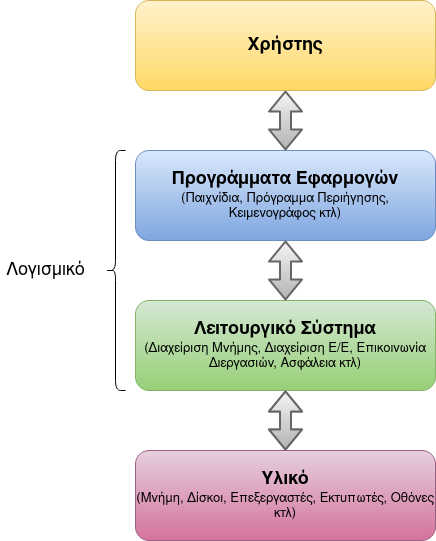
\includegraphics[scale=0.6]{images/OS_hierarchy.png}
    \caption{Δομή Υλικού και Λογισμικού Υπολογιστή}
    \label{fig:os_hierarchy}
\end{figure}

Το ΛΣ, επομένως, <<κάθεται>> ανάμεσα στο υλικό και στις εφαρμογές που χρησιμοποιεί ο χρήστης ο οποίος συνήθως δεν ενδιαφέρεται για λεπτομέρειες του υλικού του υπολογιστή. Δρα, δηλαδή, ως ένας διαμεσολαβητής που διευκολύνει την επικοινωνία του χρήστη με τον υπολογιστή χωρίς ο πρώτος να χρειάζεται να γνωρίζει την γλώσσα του τελευταίου, ενώ είναι υπεύθυνο για την ομαλή λειτουργία των προγραμμάτων εφαρμογών. Για παράδειγμα, προκειμένου να εμφανιστεί το κείμενο <<Χαίρε Κόσμε>> στην οθόνη, πρέπει μερικές εκατοντάδες πίξελ να λειτουργήσουν σε συγκεκριμένες θέσεις. Αυτό μπορεί να γίνει με το να διαβάζει κανείς τις προδιαγραφές του υλικού και να γράψει κώδικα που χειρίζεται τα σωστά μπιτς στην μνήμη κάτι που είναι αρκετά επίπονο. Οι περισσότεροι χρήστες όμως θέλουν απλά να γράψουν την εντολή \texttt{\selectlanguage{english}print("Hello World")} χωρίς να νοιαστούν για περαιτέρω λεπτομέρειες. Εκεί είναι που μπαίνει το ΛΣ για να δώσει λύση \cite{elements_of_computing}.

Πιο αναλυτικά, μερικές από τις περιοχές στις οποίες το ΛΣ παρέχει υπηρεσίες περιγράφονται παρακάτω σύμφωνα με το \cite{stallings}:

\begin{itemize}
    \item \textbf{Στην ανάπτυξη προγραμμάτων:} Το ΛΣ παρέχει πληθώρα υπηρεσιών, όπως επεξεργαστές κειμένου και διορθωτές λαθών ({\selectlanguage{english}debuggers}), προκειμένου να βοηθήσει τον προγραμματιστή στην ανάπτυξη εφαρμογών. Συνήθως, οι υπηρεσίες αυτές έχουν τη μορφή βοηθητικών προγραμμάτων, τα οποία αν και δεν αποτελούν αυστηρά τμήμα του πυρήνα του λειτουργικού συστήματος, παρέχονται μαζί με το ΛΣ και αναφέρονται ως εργαλεία ανάπτυξης προγραμμάτων εφαρμογών.
    \item \textbf{Στην εκτέλεση προγραμμάτων:} Για την εκτέλεση ενός προγράμματος απαιτείται πλήθος βημάτων. Εντολές και δεδομένα πρέπει να φορτωθούν στην κύρια μνήμη, συσκευές Εισόδου/Εξόδου (Ε/Ε) και αρχεία πρέπει να αρχικοποιηθούν και διάφοροι άλλοι πόροι πρέπει να ετοιμαστούν. Το ΛΣ διαχειρίζεται αυτές τις υποχρεώσεις χρονοδρομολόγησης για λογαριασμό του χρήστη.
    \item \textbf{Στην πρόσβαση σε συσκευές Εισόδου/Εξόδου(Ε/Ε):} Κάθε συσκευή Ε/Ε απαιτεί το δικό της ιδιαίτερο σύνολο εντολών ή σημάτων ελέγχου για τη λειτουργία της. Το ΛΣ παρέχει ενιαία διεπαφή που αποκρύπτει αυτές τις λεπτομέρειες, έτσι ώστε οι προγραμματιστές να έχουν πρόσβαση σε τέτοιες συσκευές χρησιμοποιώντας απλές αναγνώσεις ({\selectlanguage{english}reads}) και εγγραφές ({\selectlanguage{english}writes}).
    \item \textbf{Στην ελεγχόμενη πρόσβαση σε αρχεία:} Το ΛΣ πρέπει να αναπαριστά τη λεπτομερή κατανόηση, όχι μόνο της φύσης των συσκευών Ε/Ε (οδηγού δίσκου, οδηγού ταινίας), αλλά και της δομής των δεδομένων που βρίσκονται σε αρχεία στο αποθηκευτικό μέσο. Επίσης, στην περίπτωση συστημάτων πολλαπλών χρηστών, το ΛΣ μπορεί να παρέχει μηχανισμούς προστασίας για τον έλεγχο της πρόσβασης σε αρχεία.
    \item \textbf{Στην πρόσβαση στο σύστημα:} Σε ό,τι αφορά διαμοιραζόμενα ή δημόσια συστήματα, το ΛΣ ελέγχει συνολικά την πρόσβαση στο σύστημα και σε συγκεκριμένους πόρους του. Η λειτουργία πρόσβασης πρέπει να παρέχει προστασία των πόρων και των δεδομένων από μη εξουσιοδοτημένους χρήστες και να διευθετεί θέματα συγκρούσεων και διεκδίκησης πόρων.
    \item \textbf{Στην ανίχνευση σφαλμάτων και στην απόκριση:} Διάφορα σφάλματα μπορούν να προκύψουν κατά τη διάρκεια λειτουργίας ενός υπολογιστικού συστήματος. Μεταξύ αυτών περιλαμβάνονται εσωτερικά και εξωτερικά σφάλματα υλικού, όπως σφάλματα μνήμης ή δυσλειτουργία κάποιας συσκευής, καθώς και διάφορα σφάλματα λογισμικού, όπως η διαίρεση με το μηδέν και η προσπάθεια προσπέλασης απαγορευμένης θέσης μνήμης. Σε κάθε περίπτωση, το ΛΣ πρέπει να παρέχει μια απόκριση, η οποία απαλείφει τη συνθήκη σφάλματος, με το μικρότερο δυνατό αντίκτυπο στις εφαρμογές που εκείνη την ώρα εκτελούνται. Απόκριση μπορεί να αποτελεί η λήξη του προγράμματος που προκάλεσε το σφάλμα, η επανέναρξη λειτουργίας ή ακόμα και η απλή αναφορά σφάλματος στην εφαρμογή.
    \item \textbf{Στην λογιστική:} Ένα καλό ΛΣ συλλέγει στατιστικά χρήσης διάφορων πόρων και παρακολουθεί παραμέτρους απόδοσης, όπως είναι ο χρόνος απόκρισης. Σε κάθε σύστημα, οι πληροφορίες αυτές είναι χρήσιμες για τη λήψη αποφάσεων σχετικών με μελλοντικές αναβαθμίσεις και με τις ρυθμίσεις του συστήματος, ώστε να επιτυγχάνεται η βελτίωση της απόδοσης. Σε συστήματα πολλαπλών χρηστών, οι πληροφορίες αυτές μπορούν να χρησιμοποιηθούν και για λόγους χρέωσης.
\end{itemize}
\subsection{Το ΛΣ ως Διαχειριστής Πόρων}
Όπως αναφέρεται και παραπάνω το ΛΣ είναι μεταξύ άλλων υπεύθυνο για τον έλεγχο των πόρων του υπολογιστή, δηλαδή τις μνήμες, τους δίσκους, τον επεξεργαστή κτλ. Αναφέρθηκε, επίσης, ότι το ΛΣ είναι και αυτό ένα λογισμικό και άρα λειτουργεί με τον ίδιο τρόπο που λειτουργεί οποιαδήποτε άλλη εφαρμογή, δηλαδή είναι μια ακολουθία εντολών που εκτελούνται από τον επεξεργαστή. Κατά την φάση εκτέλεσης, το ΛΣ κατανέμει τον χρόνο του επεξεργαστή και τους πόρους του υπολογιστή στα προγράμματα που πρόκειται να τρέξουν. Για να εκτελεστεί όμως μια εφαρμογή ή ένα πρόγραμμα ο επεξεργαστής πρέπει να διακόψει την εκτέλεση του ΛΣ, ενώ μετά το πέρας των εντολών επαναφέρει το ΛΣ στον έλεγχο προκειμένου να γίνουν οι απαραίτητες προετοιμασίες για τις επόμενες εργασίες \cite{stallings}.

Ακριβώς επειδή το ΛΣ βοηθάει την εκτέλεση σχεδόν κάθε προγράμματος πρέπει να είναι και αρκετά αποδοτικό. Για παράδειγμα, τα προγράμματα εφαρμογών δημιουργούν αντικείμενα και πίνακες συνέχεια οπότε είναι σημαντικό αυτή η δουλειά να γίνεται γρήγορα και με εξοικονόμηση πόρων. Οποιοδήποτε κέρδος του ΛΣ, είτε σε ταχύτητα είτε σε μνήμη, μπορεί να επηρεάσει δραματικά την απόδοση του υπολογιστικού συστήματος \cite{elements_of_computing}.

\section{\texorpdfstring{\engl{Open Graphics Library}}{Open Graphics Library}}
Αντίστοιχα με το ΛΣ αλλά ανεξάρτητο από αυτό, η \textbf{\selectlanguage{english}Open Graphics Library}\cite{opengl_specification} (εν συντομία \textbf{\selectlanguage{english}OpenGL}) αποτελεί μία \textsl{Διεπαφή Προγραμματισμού Εφαρμογών} για τη βέλτιστη χρήση των πόρων της κάρτας γραφικών με σκοπό την οικονομική και γρήγορη απόδοση {\selectlanguage{english}2D} και {\selectlanguage{english}3D} γραφικών. Η διεπαφή περιλαμβάνει ένα σύνολο εντολών οι οποίες επιτρέπουν στον χρήστη να καθορίσει τα απαραίτητα αντικείμενα και διεργασίες για την παραγωγή υψηλής ποιότητας έγχρωμων εικόνων δισδιάστατων ή τρισδιάστατων αντικειμένων.

\subsection{Αρχές Λειτουργίας της \texorpdfstring{\engl{OpenGL}}{OpenGL}}
Η {\selectlanguage{english}OpenGL} είναι υπεύθυνη για την επεξεργασία των δεδομένων στην μνήμη της κάρτας γραφικών, την εγγραφή δεδομένων στον {\selectlanguage{english}framebuffer} και την ανάγνωση του. Ο {\selectlanguage{english}framebuffer} απαρτίζεται από ένα σύνολο {\selectlanguage{english}pixels} διατεταγμένων σε ένα δισδιάστατο πίνακα. Κάθε στοιχείο του πίνακα αποτελείται από έναν αριθμό {\selectlanguage{english}bits}, ανάλογα με την υλοποίηση της {\selectlanguage{english}OpenGL}, τα οποία καθορίζουν το χρώμα, το βάθος και το στένσιλ για κάθε {\selectlanguage{english}pixel}.

Στο Σχήμα \ref{fig:opengl_pipeline} φαίνεται η διαδικασία απεικόνισης γραφικών της {\selectlanguage{english}OpenGL}. Αρχικά, δέχεται ως είσοδο τα δεδομένα των κορυφών των αντικειμένων προς προβολή, τα οποία συνθέτονται σε πρωτόγονα σχήματα όπως κορυφές, τμήματα γραμμών, επιφάνειες και πολύγωνα. Στη συνέχεια, οι κορυφές μεταμορφώνονται σε γεωμετρικά πρωτόγονα σχήματα, συνήθως τρίγωνα ή πολύγωνα, τα οποία μέσω ψηφίδωσης μπορούν να παράξουν περισσότερα πρωτόγονα σχήματα από μία είσοδο. Προαιρετικά, τα αποτελέσματα από αυτά τα στάδια δύναται να ανατροφοδοτήσουν ενδιάμεσες μνήμες για μετέπειτα χρήση.

\begin{figure}[t]
    \centering
    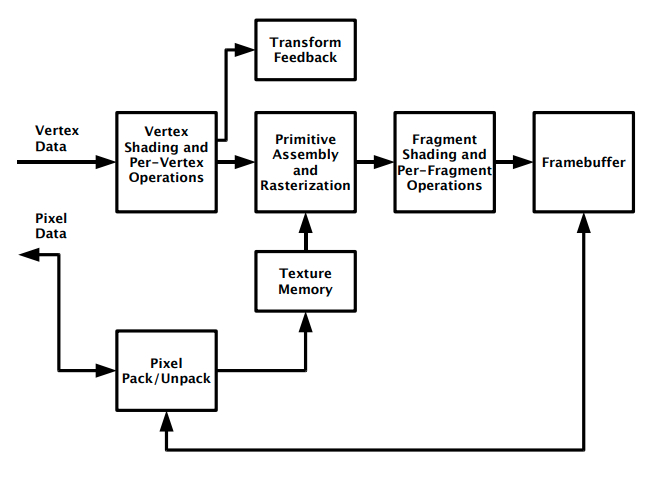
\includegraphics[scale=2.2]{images/opengl_pipeline.jpg}
    \caption{Διαδικασία απεικόνισης γραφικών της {\selectlanguage{english}OpenGL}}
    \label{fig:opengl_pipeline}
\end{figure}

Τα τελικά πρωτόγονα σχήματα περικόπτονται από έναν καθορισμένο όγκο για να προετοιμαστούν για το στάδιο της ψηφιοποίησης. Η διαδικασία αυτή παράγει σειρές από διευθύνσεις του {\selectlanguage{english}framebuffer} συνοδευόμενες από τιμές που περιγράφουν τη δισδιάστατη απεικόνιση των αρχικών τρισδιάστατων πρωτόγονων σχημάτων. Κάθε τμήμα που παράγεται με αυτό τον τρόπο υπόκειται σε περαιτέρω διεργασίες ξεχωριστά. Οι διεργασίες περιλαμβάνουν υπό συνθήκη ενημέρωση των τιμών σε συνάρτηση με εισερχόμενες ή αποθηκευμένες τιμές του βάθους ή του στένσιλ, ανάμειξη των εισερχόμενων χρωμάτων με αποθηκευμένα χρώματα ή άλλες λογικές πράξεις στις τιμές των τμημάτων. Τέλος, ο {\selectlanguage{english}framebuffer} επικαιροποιείται με τις τιμές των τμημάτων, προβάλλοντας έτσι την τελική εικόνα στην οθόνη.

%%% ΙοΤ %%%
\section{Διαδίκτυο των Πραγμάτων}
Το \textbf{Διαδίκτυο των Πραγμάτων} (μτφ. \textbf{\selectlanguage{english}Internet of Things}, εν συντομία \textbf{ΙοΤ}) είναι ένα σύνολο φυσικών αντικειμένων τα οποία έχουν αισθητήρες, λογισμικό, υπολογιστική ισχύ κτλ. και τα οποία ανταλλάσσουν δεδομένα μεταξύ τους μέσω του Διαδικτύου ή ενός οποιουδήποτε άλλου δικτύου επικοινωνίας. Τα αντικείμενα αυτά μπορεί να είναι ένας άνθρωπος με βηματοδότη στην καρδιά, ένα έξυπνο ρολόι που μετράει παλμούς, ένας καθρέφτης που διαβάζει δεδομένα από αισθητήρες και εμφανίζει πληροφορίες για την κατάσταση του χρήστη.

\subsection{Πώς δουλεύει το ΙοΤ}
Ένα σύστημα ΙοΤ περιέχει πολλές φυσικές μονάδες ({\selectlanguage{english}hardware}) οι οποίες μπορούν να χωριστούν στις ακόλουθες κατηγορίες {\cite{chebudie}}:
\begin{itemize}
    \item Αισθητήρες \& Ενεργοποιητές (\engl{Sensors \& Actuators})
    \item Μονάδες Επεξεργασίας (\engl{Processing Units})
    \item Μονάδες Αποθήκευσης (\engl{Storage Units})
    \item Μονάδες Επικοινωνίας (\engl{Communication Units})
\end{itemize}

Σε ό,τι αφορά το λογισμικό των ΙοΤ συσκευών, δεν υπάρχει κάποια συγκεκριμένη αρχιτεκτονική που να ακολουθείται καθολικά. Έχουν προταθεί αρκετές, ενώ παρακάτω παρουσιάζονται 2 από τις πιο διαδεδομένες, η αρχιτεκτονική 3 επιπέδων και η αρχιτεκτονική 5 επιπέδων \cite{sethi}.

\subsubsection{Αρχιτεκτονική 3 επιπέδων}
Η αρχιτεκτονική 3 επιπέδων είναι από τις πιο βασικές και πρώιμες αρχιτεκτονικές που αναπτύχθηκαν και απεικονίζεται στο Σχήμα \ref{fig:iot_3_tier}.
\begin{figure}[h]
    \centering
    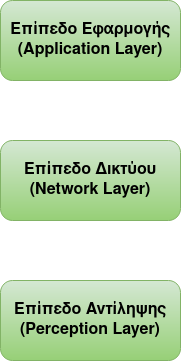
\includegraphics[scale=0.7]{images/IoT_3tier.png}
    \caption{Αρχιτεκτονική 3 Επιπέδων}
    \label{fig:iot_3_tier}
\end{figure}

Όπως προκύπτει και από το όνομα αποτελείται από 3 επίπεδα:
\begin{itemize}
    \item \textbf{Επίπεδο Αντίληψης:} Το επίπεδο αντίληψης είναι το φυσικό επίπεδο (\engl{hardware}) το οποίο περιέχει αισθητήρες για λήψη πληροφοριών και ανίχνευση παραμέτρων από τον περιβάλλοντα χώρο.
    \item \textbf{Επίπεδο Δικτύου:} Το επίπεδο δικτύου είναι υπεύθυνο για την διασύνδεση με άλλες συσκευές, έξυπνα πράγματα κτλ. Χρησιμοποιείται επίσης για την μετάδοση και επεξεργασία δεδομένων των αισθητήρων.
    \item \textbf{Επίπεδο Εφαρμογής:} Το επίπεδο εφαρμογής είναι υπεύθυνο για την παροχή υπηρεσιών συγκεκριμένης εφαρμογής (\engl{application specific services}) στον χρήστη. Καθορίζει τις διάφορες εφαρμογές στις οποίες μπορεί να αναπτυχθεί το ΙοΤ, όπως το έξυπνο σπίτι, ο έξυπνος καθρέφτης κ.α.
\end{itemize}

\subsubsection{Αρχιτεκτονική 5 επιπέδων}
Η αρχιτεκτονική των 3 επιπέδων περιγράφει την βασική ιδέα πίσω από το ΙοΤ, αλλά στην πράξη δεν επαρκή. Για το λόγο αυτό, υπάρχουν αρχιτεκτονικές με περισσότερα επίπεδα στην βιβλιογραφία. Μία από αυτές είναι η αρχιτεκτονική 5 επιπέδων που φαίνεται στο Σχήμα \ref{fig:iot_5_tier}.

\begin{figure}[h]
    \centering
    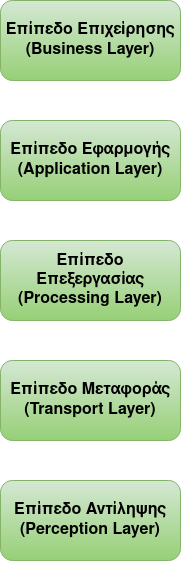
\includegraphics[scale=0.7]{images/IoT_5tier.png}
    \caption{Αρχιτεκτονική 5 Επιπέδων}
    \label{fig:iot_5_tier}
\end{figure}

Στην περίπτωση αυτή, τα επίπεδα Αντίληψης και Εφαρμογής παραμένουν ίδια με αυτά της αρχιτεκτονικής 3 επιπέδων ενώ επεξηγούνται και τα υπόλοιπα 3 επίπεδα:
\begin{itemize}
    \item \textbf{Επίπεδο Μεταφοράς:} Το επίπεδο μεταφοράς, μεταδίδει τα δεδομένα των αισθητήρων από το επίπεδο αντίληψης στο επίπεδο επεξεργασίας και αντίστροφα μέσω δικτύων όπως \engl{3G, LAN, RFID, NFC }κτλ.
    \item \textbf{Επίπεδο Επεξεργασίας:} Το επίπεδο επεξεργασίας, γνωστό και ως \engl{middleware}, αποθηκεύει, αναλύει και επεξεργάζεται μεγάλο όγκο δεδομένων που προέρχονται από το επίπεδο μεταφοράς. Προσφέρει μια ευρεία γκάμα υπηρεσιών στα χαμηλότερα επίπεδα. Χρησιμοποιεί επίσης πολλές τεχνολογίες όπως βάσεις δεδομένων, υπολογιστική νέφους και ενότητες επεξεργασίας μεγάλων δεδομένων.
    \item \textbf{Επίπεδο Επιχείρησης:} Το επίπεδο επιχείρησης διαχειρίζεται όλο το ΙοΤ σύστημα, συμπεριλαμβανομένων των εφαρμογών του, των επιχειρηματικών του μοντέλων και της ιδιωτικότητας των χρηστών.
\end{itemize}


\newpage
\section{Ανάπτυξη Λογισμικού}

Στη σύγχρονη πραγματικότητα, το λογισμικό έχει κυριαρχήσει στην καθημερινή ζωή, καθιστώντας το μία από τις σημαντικότερες τεχνολογίες. Παίζοντας ταυτόχρονα το ρόλο προϊόντος και εργαλείου, αποτελεί τη βάση της επιστημονικής έρευνας και της επίλυσης προβλημάτων μηχανικής, καθιστώντας δυνατή την δημιουργία καινούργιων και την επέκταση υπαρχουσών τεχνολογιών (π.χ. γενετική μηχανική και τηλεπικοινωνίες αντίστοιχα). Ταυτόχρονα, έχει διεισδύσει σε συστήματα κάθε είδους: μεταφοράς, ιατρικά, τηλεπικοινωνιών, στρατιωτικά, βιομηχανικά, ψυχαγωγίας κ.α. αλλάζοντας τον τρόπο που αντιλαμβανόμαστε και αλληλεπιδράμε με τον κόσμο.

Έτσι, τα λογισμικά προγράμματα αντιμετωπίζουν ολοένα και περισσότερα προβλήματα της καθημερινής ζωής, αυξάνοντας την αναγκαιότητα και το κόστος τους. Πράγματι, το συνολικό κόστος λογισμικού υπολογίζεται στα \euro500 δισεκατομμύρια στην Αμερική και διπλάσιο παγκοσμίως \cite{software_engineering_principles}. Αυτό αναφέρεται τόσο στο κόστος ανάπτυξης του λογισμικού όσο και συντήρησής του αφού έχει παραδοθεί στον πελάτη. Ταυτόχρονα, το κόστος του υλικού έχει μειωθεί δραματικά, αποτελώντας λιγότερο από το 20\% των συνολικών εξόδων ενός συστήματος όπως φαίνεται στο Σχήμα \ref{fig:hardware_software_costs}.

\begin{figure}[h]
    \centering
    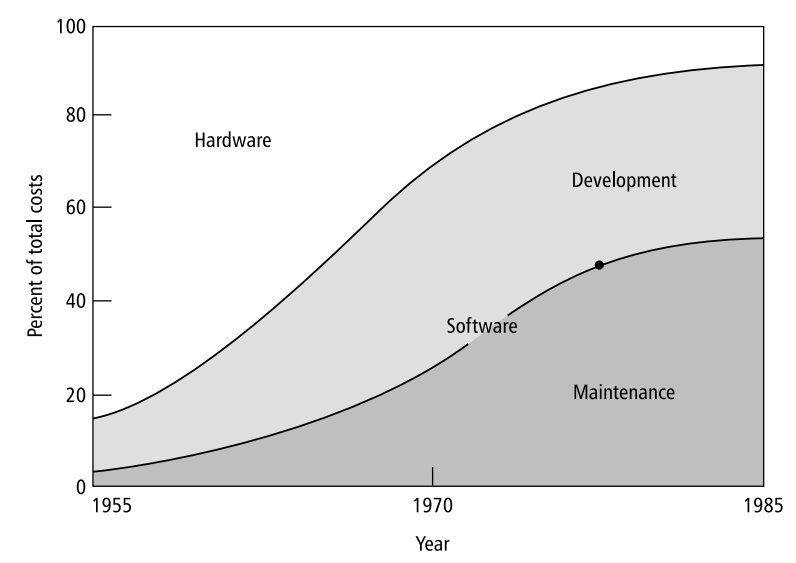
\includegraphics[scale=2.2]{images/software_engineering/hardware_software_costs.png}
    \caption{Σχετική κατανομή κόστους υλικού/λογισμικού (\textsl{Πηγή: \cite{hardware_software_costs}}) }
    \label{fig:hardware_software_costs}
\end{figure}

Η διαφορά κόστους έγκειται στο γεγονός ότι τα σύγχρονα προγράμματα λογισμικού είναι μεγάλα και περίπλοκα, απαιτώντας ομάδες υψηλής εξειδίκευσης, δεν έχουν περιορισμούς (δηλαδή έχουν περισσότερους βαθμούς ελευθερίας) και τέλος επειδή υφίσταται συνεχόμενες αλλαγές. Μάλιστα, στη διάρκεια ζωής του λογισμικού οι αλλαγές αυτές ενδέχεται να εισάγουν σφάλματα, αυξάνοντας τον κίνδυνο αποτυχίας του συστήματος, όπως φαίνεται στο Σχήμα \ref{fig:software_failure_rate}. Επιπλέον, σε αντίθεση με την αποτυχία του υλικού, όπου αντιμετωπίζεται με αντικατάσταση του χαλασμένου μέρους, η αποτυχία του λογισμικού έγκειται σε σφάλμα σχεδιασμού, καθιστώντας τη συντήρηση του σημαντικά πιο περίπλοκη και ακριβή διαδικασία.

\begin{figure}[h]
    \centering
    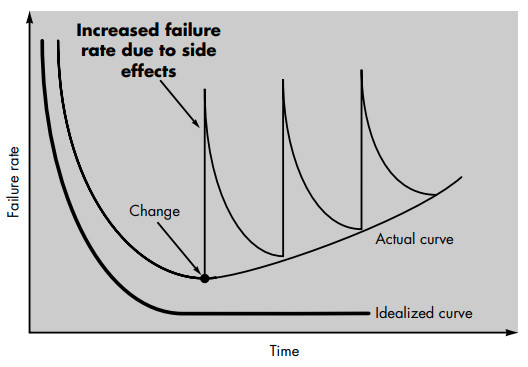
\includegraphics[scale=2.2]{images/software_engineering/software_failure_rate.jpg}
    \caption{Καμπύλη αποτυχίας για το λογισμικό}
    \label{fig:software_failure_rate}
\end{figure}

Εντούτοις, η αυξανόμενη εξάρτηση των καθημερινών δραστηριοτήτων από περίπλοκα συστήματα λογισμικού απαιτεί την εύρωστη και αλάνθαστη λειτουργία τους καθ' όλη τη διάρκεια ζωής του λογισμικού, το οποίο όμως αλλάζει συνεχώς αυξάνοντας τον κίνδυνο αποτυχίας του. Τοιουτοτρόπως, για την μείωση του ρίσκου αποτυχίας και την απλούστευση της ανάπτυξης και συντήρησης υψηλής ποιότητας έργων λογισμικού, έπρεπε να τυποποιηθούν οι μέθοδοι και διαδικασίες που διέπουν ολόκληρο τον κύκλο ζωής του. Αυτές οι μεθοδολογίες εμπεριέχονται και αναλύονται από την επιστήμη της τεχνολογίας λογισμικού.

\subsection{Τεχνολογία Λογισμικού}

Η τεχνολογία λογισμικού είναι η συστηματική, πειθαρχημένη και μετρήσιμη προσέγγιση με σκοπό την ανάπτυξη, λειτουργία και συντήρηση υψηλής ποιότητας έργων λογισμικού. Οι διαδικασίες της τεχνολογίας λογισμικού παρέχουν ένα ευρύτερο πλαίσιο, μέσα στο οποίο εφαρμόζονται οι τεχνικές μέθοδοι, παράγονται προϊόντα δουλειάς (μοντέλα, έγγραφα, δεδομένα, αναφορές κ.α.), εξακριβώνονται σημεία σταθμοί, εξασφαλίζεται η ποιότητα και γίνεται κατάλληλη διαχείριση των αλλαγών των απαιτήσεων.

Οι μέθοδοι της τεχνολογίας λογισμικού είναι το τεχνικό εγχειρίδιο για την ανάπτυξη λογισμικού. Οι μέθοδοι εγκολπώνουν ένα ευρύ σύνολο λειτουργιών συμπεριλαμβανομένων την ανάλυση απαιτήσεων, σχεδιασμού, δημιουργία προγράμματος, δοκιμής και υποστήριξης. Οι μέθοδοι της τεχνολογίας λογισμικού βασίζονται σε βασικές αρχές και πρακτικές που διέπουν κάθε τομέα της τεχνολογίας και περιλαμβάνουν δραστηριότητες μοντελοποίησης και άλλες περιγραφικές τεχνικές.

\subsubsection{Πλαίσιο διαδικασίας}

Το πλαίσιο διαδικασίας της τεχνολογίας λογισμικού απαρτίζεται από δραστηριότητες που είναι κοινές για οποιοδήποτε έργο λογισμικού ανεξάρτητα από το μέγεθος και την περιπλοκότητα του. Ένα γενικό πλαίσιο διαδικασίας περιλαμβάνει πέντε κύριες δραστηριότητες \cite{software_engineering_practiotioner_approach}:

\begin{itemize}
    \item \textbf{Επικοινωνία} (\engl{Communication}): Πριν την έναρξη οποιασδήποτε τεχνικής εργασίας, είναι άκρως σημαντική η επικοινωνία και συνεργασία με τον πελάτη (και άλλα ενδιαφερόμενα μέλη). Η πρόθεση είναι η κατανόηση των στόχων των ενδιαφερόμενων μελών για το έργο λογισμικού και η συλλογή απαιτήσεων, βοηθώντας τον καθορισμό των λειτουργιών και των χαρακτηριστικών του λογισμικού.
    \item \textbf{Προγραμματισμός} (\engl{Planning}): Ένα έργο λογισμικού είναι ένα περίπλοκο ταξίδι και η διαδικασία του προγραμματισμού είναι ο χάρτης ο οποίος οδηγεί την ομάδα ανάπτυξης. Το σχέδιο του έργου αποσαφηνίζει την απαιτούμενη δουλειά, περιγράφοντας τις τεχνικές εργασίες προς διεκπεραίωση, τα πιθανά ρίσκα, τους απαιτούμενους πόρους, τα προϊόντα προς παραγωγή και το πρόγραμμα εργασίας. 
    \item \textbf{Μοντελοποίηση} (\engl{Modelling}): Δημιουργούνται μοντέλα ώστε να γίνει εφικτή η καλύτερη κατανόηση των απαιτήσεων του λογισμικού και του σχεδιασμού ο οποίος δύναται να ικανοποιήσει αυτές τις απαιτήσεις. Γίνεται εμφανής η αρχιτεκτονική μορφή του έργου, ο τρόπος αλληλεξάρτησης των μεμονωμένων μερών και πολλά άλλα χαρακτηριστικά, στη προσπάθεια κατανόησης του προβλήματος και του τρόπου επίλυσης του.
    \item \textbf{Κατασκευή} (\engl{Construction}): Η δραστηριότητα αυτή περιλαμβάνει την υλοποίηση του έργου παράγοντας κώδικα (είτε με χειροκίνητο ή αυτόματο τρόπο) και τον έλεγχο του κώδικα για την ανίχνευση σφαλμάτων. 
    \item \textbf{Εγκατάσταση} (\engl{Deployment}): Το λογισμικό ως ολόκληρη οντότητα ή σε επιμέρους διαδοχικά στάδια παραδίνεται στον πελάτη ο οποίος αξιολογεί το παραδοθέν προϊόν και παρέχει ανατροφοδότηση.
\end{itemize}

Σε πολλά έργα λογισμικού, οι δραστηριότητες πλαισίου εφαρμόζονται επαναληπτικά καθώς αναπτύσσεται το έργο. Κάθε επανάληψη παράγει μία επαύξηση του λογισμικού η οποία θέτει στην διάθεση των ενδιαφερόμενων μελών ένα υποσύνολο των τελικών χαρακτηριστικών και λειτουργιών του λογισμικού. Τοιουτοτρόπως, το λογισμικό ολοκληρώνεται σταδιακά με το πέρας κάθε επανάληψης. 

\subsection{Ροές διαδικασίας Τεχνολογίας Λογισμικού}

Μία διαδικασία ορίζεται ως το άθροισμα των δραστηριοτήτων, ενεργειών και εργασιών που πρέπει να διεκπεραιωθούν με σκοπό την παραγωγή ενός προϊόντος εργασίας. Όπως αναφέρθηκε παραπάνω, το γενικό πλαίσιο διαδικασίας του λογισμικού αποτελείται από πέντε δραστηριότητες σε συνδυασμό με άλλες ενέργειες - όπως παρακολούθηση και έλεγχος έργου, εκτίμηση και διαχείριση ρίσκου, διασφάλιση ποιότητας, ρύθμιση παραμέτρων κ.α. - που εφαρμόζονται καθ' όλη την διαδικασία.

Η ροή διαδικασίας περιγράφει τον τρόπο με τον οποίο οι δραστηριότητες πλαισίου, οι ενέργειες και οι εργασίες εντός κάθε δραστηριότητας οργανώνονται σε σχέση με την αλληλουχία τους και τον χρόνο όπως φαίνεται στο Σχήμα \ref{fig:software_process_flow}.

\begin{figure}[h]
    \begin{subfigure}{\linewidth}
        \centering
        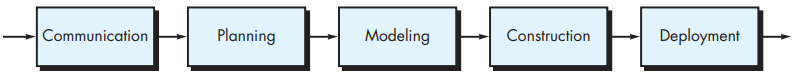
\includegraphics[scale=0.5]{images/software_engineering/linear_process_flow.png}
        \caption{Γραμμική ροή}
        \label{subfig:linear_flow}
    \end{subfigure}\par\medskip
    \begin{subfigure}{\linewidth}
        \centering
        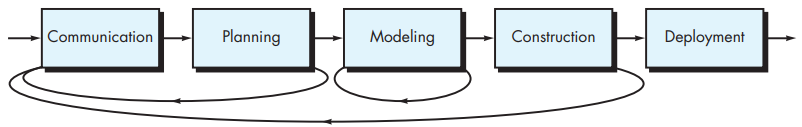
\includegraphics[scale=0.5]{images/software_engineering/iterative_process_flow.png}
        \caption{Επαναληπτική ροή}
        \label{subfig:iterative_flow}
    \end{subfigure}\par\medskip
    \begin{subfigure}{\linewidth}
        \centering
        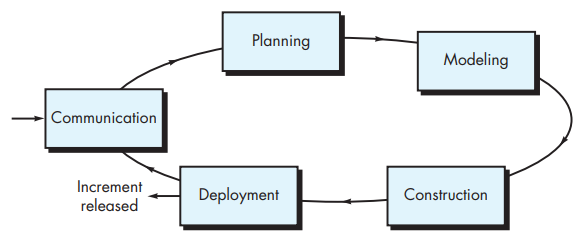
\includegraphics[width=0.7\linewidth]{images/software_engineering/evolutionery_process_flow.png}
        \caption{Εξελικτική ροή}
        \label{subfig:evolutionery_flow}
    \end{subfigure}
    \begin{subfigure}{\linewidth}
        \centering
        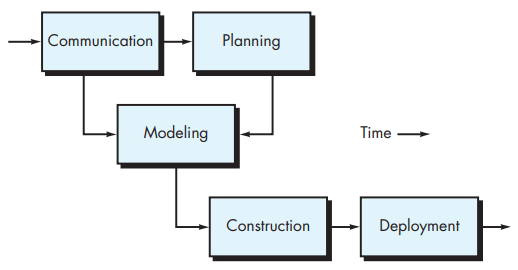
\includegraphics[width=0.7\linewidth]{images/software_engineering/parallel_process_flow.png}
        \caption{Παράλληλή ροή}
        \label{subfig:parallel_flow}
    \end{subfigure}
    \caption{Ροές διαδικασίας λογισμικού}
    \label{fig:software_process_flow}
\end{figure}

H γραμμική ροή εκτελεί τις δραστηριότητες διαδοχικά, ξεκινώντας την κάθε δραστηριότητα με το πέρας της προηγούμενης (\ref{subfig:linear_flow}). Η επαναληπτική ροή επαναλαμβάνει μία ή περισσότερες δραστηριότητες πριν προχωρήσει στην επόμενη (\ref{subfig:iterative_flow}).H εξελικτική ροή εκτελεί τις δραστηριότητες κυκλικά. Στο πέρας της διεκπεραίωσης των δραστηριοτήτων παράγεται σταδιακά η εφαρμογή ολοένα και πιο ολοκληρωμένη (\ref{subfig:evolutionery_flow}). Η παράλληλη ροή (\ref{subfig:parallel_flow}) εκτελεί μία ή περισσότερες δραστηριότητες παράλληλα με άλλες δραστηριότητες (για παράδειγμα η μοντελοποίηση μιας πτυχής του λογισμικού μπορεί να γίνεται ταυτόχρονα με την κατασκευή μιας άλλης πτυχής του).

\subsection{Μοντέλα ανάπτυξης λογισμικού}

\subsubsection{Μοντέλο Καταρράκτη}

Το μοντέλο ανάπτυξης \textsl{καταρράκτη} ακολουθεί την γραμμική ροή, δηλαδή οι δραστηριότητες από την \textsl{επικοινωνία} μέχρι την \textsl{εγκατάσταση} διεκπεραιώνονται διαδοχικά. Το μοντέλο αυτό επιλέγεται όταν οι απαιτήσεις του λογισμικού είναι ξεκάθαρα ορισμένες και επαρκώς σταθερές.

Το μοντέλο \textsl{καταρράκτη} είναι το παλαιότερο μοντέλο της τεχνολογίας λογισμικού. Εντούτοις, με την εξέλιξη της τεχνολογίας και των απαιτήσεων έχει παρουσιάσει πληθώρα προβλημάτων.

\begin{itemize}
  \item Τα έργα λογισμικού σπάνια ακολουθούν την προτεινόμενη γραμμική ροή. Τοιουτοτρόπως, οι αλλαγές δεν είναι εύκολα διαχειρίσιμες και μπορεί να προκαλέσουν σύγχυση. 
  \item Συνήθως είναι δύσκολο για τον πελάτη να καθορίσει όλες τις απαιτήσεις αναλυτικά. Το μοντέλο \textsl{καταρράκτη} όμως το απαιτεί και έτσι δεν μπορεί να διαχειριστεί την αβεβαιότητα που έγκειται στην έναρξη οποιουδήποτε έργου λογισμικού.
  \item Μία λειτουργική έκδοση του λογισμικού γίνεται διαθέσιμη αρκετά αργά στην διάρκεια ζωής του έργου. Έτσι, από την μία ο πελάτης πρέπει να είναι υπομονετικός και από την άλλη μία αστοχία σχεδιασμού που θα ανιχνευτεί κατά την αξιολόγηση της λειτουργικής έκδοσης μπορεί να είναι καταστροφική.
\end{itemize}

\subsubsection{Αυξητικό Μοντέλο}

Το \textsl{αυξητικό} μοντέλο συνδυάζει την γραμμική και την παράλληλη ροή διαδικασιών. Όπως φαίνεται στο Σχήμα \ref{fig:incremental_process_model}, το αυξητικό μοντέλο χωρίζει τις λειτουργίες και τα χαρακτηριστικά του λογισμικού σε μικρές επαυξήσεις και για κάθε επαύξηση διεκπεραιώνει γραμμικά τις δραστηριότητες, στο πέρας των οποίων παραδίδεται η λειτουργία του λογισμικού.

\begin{figure}[h]
    \centering
    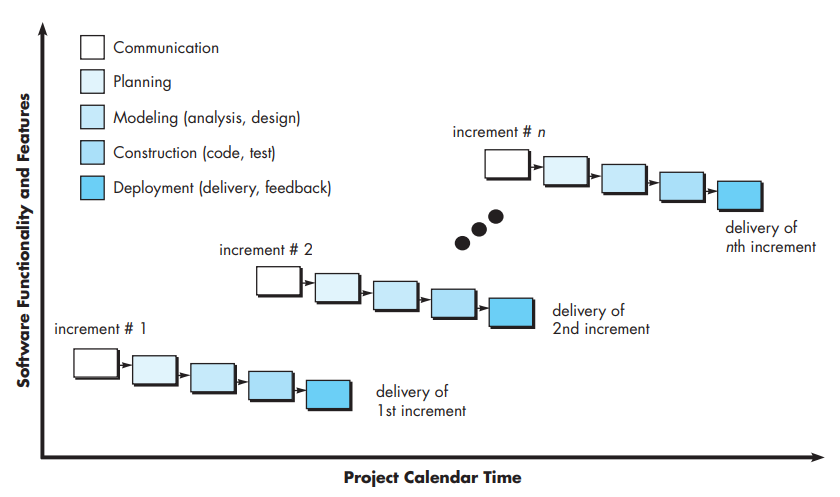
\includegraphics[scale=2]{images/software_engineering/incremental_process_model.png}
    \caption{Αυξητικό Μοντέλο}
    \label{fig:incremental_process_model}
\end{figure}

Οι πρώτες επαυξήσεις υλοποιούν τις κυριότερες λειτουργίες του λογισμικού, ικανοποιώντας τις αρχικές απαιτήσεις. Το προϊόν παραδίδεται στον πελάτη ή υπόκειται σε λεπτομερή αξιολόγηση. Τοιουτοτρόπως, αναπτύσσεται ένα σχέδιο για τις επόμενες επαυξήσεις. Το σχέδιο αφορά τις αλλαγές του κύριου προϊόντος, με σκοπό την καλύτερη ικανοποίηση των απαιτήσεων του πελάτη, και την ανάπτυξη επιπλέον χαρακτηριστικών και λειτουργιών. Η διαδικασία επαναλαμβάνεται μετά από την παράδοση κάθε επαύξησης έως ότου ολοκληρωθεί το λογισμικό.

Το αυξητικό μοντέλο είναι ιδανικό όταν υπάρχουν κάποιες πλήρης και καλά καθορισμένες απαιτήσεις με χαλαρά συζευγμένα μέρη. Έτσι, οι αρχικές επαυξήσεις μπορούν να προγραμματιστούν και να παραλληλοποιηθούν επαρκώς.

\subsubsection{Σπειροειδές Μοντέλο}

Το \textsl{σπειροειδές} μοντέλο είναι ένα εξελικτικό μοντέλο με κύριο γνώμονα το ρίσκο. Όπως και στο \textsl{αυξητικό} μοντέλο το λογισμικό παραδίδεται σε επαναλήψεις, όμως σε αντίθεση με αυτό τα βήματα δεν είναι δραστηριότητες αλλά φάσεις, με σκοπό την αντιμετώπιση του προβλήματος με το μεγαλύτερο ρίσκο να προκαλέσει αποτυχία.

\begin{figure}[h]
    \centering
    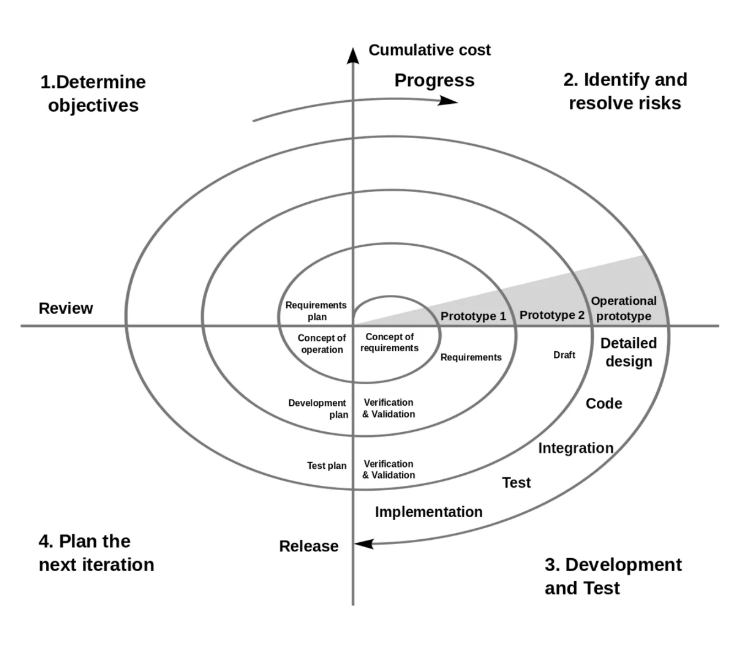
\includegraphics[scale=2]{images/software_engineering/spiral_process_model.png}
    \caption{Σπειροειδές Μοντέλο}
    \label{fig:spiral_process_model}
\end{figure}

Όπως φαίνεται στο Σχήμα \ref{fig:spiral_process_model}, οι φάσεις σε κάθε επανάληψη είναι:
\begin{enumerate}
    \item Εξακρίβωση του προβλήματος με το μεγαλύτερο ρίσκο, καθορισμός των στόχων και εναλλακτικών λύσεων.
    \item Αξιολόγηση των εναλλακτικών και προσδιορισμός των ρίσκων, σχεδιασμός των πιθανών λύσεων.
    \item Ανάπτυξη μίας λύσης, επιβεβαίωση καταλληλότητας και δοκιμή της
    \item Προετοιμασία για την επόμενη επανάληψη με βάση την ανατροφοδότηση από την παραδοθείσα επαύξηση.
\end{enumerate}

Το σπειροειδής μοντέλο μπορεί να διαχειριστεί την αβεβαιότητα εξαιρετικά καλά. Έτσι, είναι ιδανικό για έργα λογισμικού με ασαφή απαιτήσεις και για έργα που βρίσκονται στην έρευνα και ανάπτυξη.

\subsubsection{Ευέλικτο Μοντέλο}
Στη σύγχρονη πραγματικότητα, η εργασία στην παραγωγή λογισμικού έχει ταχύς ρυθμούς και είναι υποκείμενο σε συνεχή ροή αλλαγών (χαρακτηριστικών, λειτουργιών και πληροφοριακού περιεχόμενου). Έτσι, το \textsl{ευέλικτο} μοντέλο αποτελεί μία λογική εναλλακτική στις παραδοσιακές μεθόδους της τεχνολογίας λογισμικού. 

Το μοντέλο ενθαρρύνει συνεχόμενες επαναλήψεις από ανάπτυξη και δοκιμή των λειτουργιών. Σε κάθε επανάληψη παράγεται μία επαύξηση του λογισμικού αποτελούμενη από ένα μικρό σύνολο από λειτουργίες πλήρως ολοκληρωμένες. Επίσης, η κάθε επανάληψη είναι σχεδιασμένη ώστε να είναι μικρή, διαχειρίσιμη και ολοκληρώσιμη σε λίγες εβδομάδες. Συμπεριλαμβάνει των πελάτη στην διαδικασία της ανάπτυξης και ελαχιστοποιεί τα έγγραφα χρησιμοποιώντας ανεπίσημη επικοινωνία.

Το ευέλικτο μοντέλο αν και αποτελεί ρεαλιστική προσέγγιση στην ανάπτυξη λογισμικού, βρίσκεται σε μειονεκτική θέση όταν το λογισμικό είναι σύνθετο. Επίσης, αδυνατεί να διαχειριστεί τις μεταβιβάσεις λόγω των λίγων εγγράφων, αλλά από την άλλη μπορεί να διαχειριστεί τις μεταβαλλόμενες απαιτήσεις.

Οι πιο συνηθισμένες ευέλικτες μεθοδολογίες είναι:

\begin{itemize}
    \item \textbf{\engl{Scrum}}: Αποτελείται από επαναλήψεις που λέγονται \engl{sprints}. Κάθε \engl{sprint} διαρκεί 2 με 4 εβδομάδες και πριν την έναρξη του γίνεται προγραμματισμός. Αφού οριστούν οι δραστηριότητες και οι εργασίες για το \engl{sprint} δεν μεταβάλλονται κατά την διάρκειά του.
    \item \textbf{\engl{Extreme Programming (XP)}}: Σε αυτό το μοντέλο η επανάληψη διαρκεί 1 με 2 εβδομάδες. Χαρακτηριστικά αυτού του μοντέλου είναι ο προγραμματισμός σε ζεύγη, η ανάπτυξη οδηγούμενη από έλεγχο (\engl{test-driven development}), ο αυτοματοποιημένος έλεγχος, η απλή σχεδίασμη λογισμικού και τέλος οι μικρές εκδόσεις με συνεχόμενη ενσωμάτωση στο σύστημα.
    \item \textbf{\engl{Kanban}}: Το μοντέλο \engl{Kanban} επικεντρώνεται στην οπτικοποίηση, και αν υπάρχουν επαναλήψεις είναι πολύ μικρές. Στο πίνακα \engl{Kanban} παριστάνονται όλες οι δραστηριότητες και εργασίες του έργου, συνοδευόμενες από τα υπεύθυνα άτομα για την διεκπεραίωσή τους και την πρόοδό τους.
\end{itemize}


\subsection{Σχεδιαστικά Πρότυπα}
Πράγματι, οι σύγχρονες επιχειρήσεις στρέφονται ολοένα και περισσότερο προς τα \textsl{ευέλικτα μοντέλα} ανάπτυξης λογισμικού για την διαχείριση των μεταβαλλόμενων απαιτήσεων. Εντούτοις, τα \textsl{ευέλικτα μοντέλα} απαιτούν απλό σχεδιασμό του λογισμικού έτσι ώστε να μπορούν να επεκταθούν. Προς επίτευξη αυτού του σκοπού, καθίσταται επιτακτική η ανάγκη αναζήτησης και εφαρμογής σχεδιαστικών προτύπων.

Ο σκοπός των σχεδιαστικών προτύπων είναι να παρέχουν γενικές λύσεις σε συνηθισμένα προβλήματα του σχεδιασμού λογισμικού. Τυποποιώντας επίσημα τις λύσεις και τις σχέσεις μεταξύ τους καθίσταται

%% Εδώ χωράει και ένα κεφάλαιο για Neural Networks και Machine Learning
\section{\texorpdfstring{Εκτίμηση Πόζας}{Εκτίμηση Πόζας}}

Η εκτίμηση πόζας είναι μία διεργασία της υπολογιστικής όρασης όπου εκτιμάται η πόζα ενός αντικειμένου ή ανθρώπου σε μία εικόνα ή βίντεο. Το πρόβλημα της εκτίμησης πόζας περιλαμβάνει, επίσης, τον καθορισμό της θέσης και του προσανατολισμού της κάμερας σε σχέση με το αντικείμενο ή τον άνθρωπο.

Συνήθως αυτό γίνεται με την αναγνώριση, εκτίμηση θέσης και παρακολούθησης ενός αριθμού σημείων κλειδιών του αντικειμένου ή του ανθρώπου. Για τα αντικείμενα, αυτά μπορεί να είναι γωνίες ή άλλα σημαντικά χαρακτηριστικά ενώ για τον άνθρωπο τα σημεία κλειδιά αναπαριστούν κύριες αρθρώσεις όπως οι αγκώνες ή τα γόνατα.

Χαρακτηριστική είναι η διάκριση μεταξύ της \engl{2D} και της \engl{3D} εκτίμησης πόζας. Στην δισδιάστατη εκτίμηση πόζας εκτιμούνται οι θέσεις των σημείων στο \engl{2D} χώρο σε σχέση με το πλαίσιο της εικόνας ή του βίντεο. Αντιθέτως, η \engl{3D} εκτίμηση πόζας προβλέπει τις συντεταγμένες των σημείων κλειδιών σε ένα τρισδιάστατο σύστημα συντεταγμένων όπως φαίνεται στο Σχήμα \ref{fig:pose_estimation_example}.

\begin{figure}[h]
    \centering
    \begin{subfigure}{.5\textwidth}
      \centering
      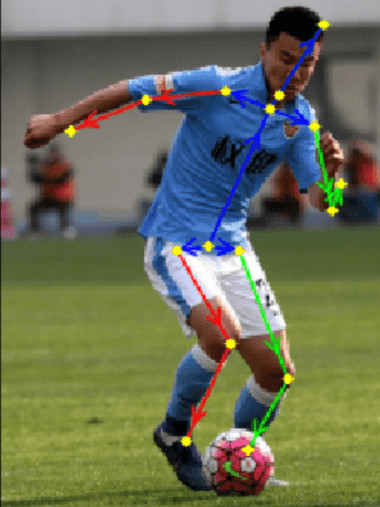
\includegraphics[width=.4\linewidth, height=4cm]{images/3d_pose_estimation/2d_estimation_example.jpg}
      \caption{\engl{2D} σημεία με συντεταγμένες $(x_i, y_i)$}
    \end{subfigure}%
    \begin{subfigure}{.5\textwidth}
      \centering
      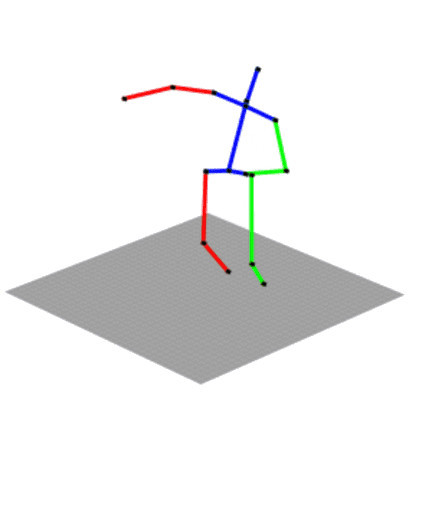
\includegraphics[width=.4\linewidth, height=4cm]{images/3d_pose_estimation/3d_estimation_example.jpg}
      \caption{\engl{3D} σημεία με συντεταγμένες $(x_i, y_i, z_i)$}
    \end{subfigure}
    \caption{Παράδειγμα εκτίμησης πόζας}
    \label{fig:pose_estimation_example}
\end{figure}

Επιπλέον, η εκτίμηση πόζας διαφοροποιείται ως προς την αναγνώριση ενός ή περισσότερων αντικειμένων. Οι δύο προσεγγίσεις αποκαλούνται μεμονωμένη εκτίμηση πόζας, όπου αναγνωρίζεται και παρακολουθείται μόνο ένα αντικείμενο ή άνθρωπος, και πολλαπλή εκτίμηση πόζας, όπου αναγνωρίζονται και παρακολουθούνται πολλαπλά.

\subsection{Μεθοδολογίες εκτίμησης πόζας}

Το πρόβλημα της εκτίμηση πόζας μπορεί να λυθεί με ποικίλους τρόπους αναλόγως με την διαρρύθμιση των αισθητήρων εικόνας και την επιλογή της μεθοδολογίας. Διακρίνονται τρεις κλάσεις μεθοδολογιών \cite{computer_vision_pose_estimation}:

\begin{itemize}
    \item \textbf{Αναλυτικές ή γεωμετρικές μέθοδοι}: Απαιτούν την ρύθμιση της κάμερας ώστε η αντιστοίχηση των τρισδιάστατων σημείων της σκηνής και των δισδιάστατων σημείων της εικόνας να είναι γνωστή. Τοιουτοτρόπως, γνωρίζοντας την γεωμετρία του αντικειμένου η προβολή του στην εικόνα της κάμερας είναι μια γνωστή συνάρτηση της πόζας του αντικειμένου. Έτσι, το πρόβλημα της εκτίμησης πόζας λύνεται αναγνωρίζοντας τα σημεία κλειδιά και στην συνέχεια λύνοντας το σύνολο των εξισώσεων που αντιστοιχίζουν τις τρισδιάστατες συντεταγμένες των σημείων με τις δισδιάστατες συντεταγμένες της εικόνας.
    \item \textbf{Γενετικοί αλγόριθμοι}: Στην περίπτωση που η πόζα του αντικειμένου ή του ανθρώπου δεν απαιτεί τον υπολογισμό της σε πραγματικό χρόνο μπορεί να χρησιμοποιηθεί ένας \textsl{γενετικός αλγόριθμος}. Η πόζα περιγράφεται από μεταβλητές, όπως για παράδειγμα οι περιστροφές των αρθρώσεων από μία στάση αναφοράς, οι οποίες χρησιμοποιούνται ως παράμετροι εισόδου του \textsl{γενετικού}, ορίζοντας έτσι τη συνάρτηση καταλληλότητας (\engl{fitness function}) ως το σφάλμα της προβολής των εκτιμώμενων τρισδιάστατων σημείων κλειδιών από τις πραγματικές συντεταγμένες τους στο δισδιάστατο πλαίσιο της εικόνας. 
    \item \textbf{Μηχανική μάθηση}: Οι μέθοδοι \textsl{μηχανικής μάθησης} χρησιμοποιούν ένα σύστημα τεχνητής νοημοσύνης το οποίο μαθαίνει την αντιστοίχηση των \engl{2D} χαρακτηριστικών της εικόνας με τις παραμέτρους μοντελοποίησης που περιγράφουν με σαφήνεια την πόζα. Εν συντομία, ένα επαρκώς μεγάλο σύνολο από φωτογραφίες ή βίντεο αντικειμένων ή ανθρώπων σε διαφορετικές πόζες χρησιμοποιείται ως είσοδος στο σύστημα κατά την διάρκεια της φάσης εκμάθησης. Με το πέρας της εκμάθησης, το σύστημα μπορεί να εκτιμήσει την πόζα του αντικειμένου ή ανθρώπου δεδομένης της \engl{2D} εικόνας του.
\end{itemize}

Στη συγκεκριμένη εφαρμογή, απαιτείται η εκτίμηση της ανθρώπινης πόζας στον τρισδιάστατο χώρο σε πραγματικό χρόνο. Το πρόβλημα αυτό κρίνεται άκρως περίπλοκο, με την δυσκολία του να έγκειται στο γεγονός ότι η εκτίμηση της τρισδιάστατης πόζας από μία δισδιάστατη εικόνα είναι εξ ορισμού κακώς ορισμένο πρόβλημα. Αυτό γίνεται εμφανές αν σκεφτούμε ότι μία δισδιάστατη πόζα μπορεί να προκύψει από πολυάριθμες τρισδιάστατες πόζες. Ταυτόχρονα, υπάρχουν πολλές επιπλέον προκλήσεις όπως η αβεβαιότητα του περιβάλλοντος, του φόντου, του φωτισμού, η κίνηση της κάμερας, οι γρήγορες κινήσεις, οι μεταβολές των ρούχων και των σκιών που μπορεί να κάνουν την μορφή και το σχήμα του ανθρώπου να αλλάζει δραματικά με την πάροδο του χρόνου. Επιπλέον, οι ανθρώπινες αρθρώσεις είναι μικρές, οριακά εμφανής και έχουν πολλούς βαθμούς ελευθερίας δυσχεραίνοντας ακόμα περισσότερο το πρόβλημα της εκτίμησης πόζας. Ως εκ τούτου, η καταλληλότερη μεθοδολογία για την επίλυση του προβλήματος είναι η \textsl{Βαθιά Μηχανική Μάθηση}, ικανοποιώντας τόσο την απαίτηση της σχετικά ακριβής εκτίμησης των σημείων κλειδιών αλλά και διεξάγοντας την εκτίμηση σε πραγματικό χρόνο. Στη συνέχεια του κεφαλαίου λοιπόν, θα αναλύσουμε το θεωρητικό υπόβαθρο που συναντάει κανείς στις διάφορες προσεγγίσεις επίλυσης του προβλήματος εκτίμησης ανθρώπινης πόζας.

\subsection{Μοντελοποίηση ανθρώπινου σώματος}

Όπως αναφέρθηκε, το ανθρώπινο σώμα είναι περίπλοκο με πολλαπλές αρθρώσεις πολλών βαθμών ελευθερίας και μεγάλου εύρους κίνησης. Τοιουτοτρόπως, κρίνεται αναγκαία η σαφής μοντελοποίηση της υποβόσκουσας δομής του, μειώνοντας αφενός την εγγενή αβεβαιότητα του προβλήματος εκτίμησης πόζας και αφετέρου αποτελώντας το μέσο για την περιγραφή της τελικής πόζας.

Οι διαφορετικές μέθοδοι εκτίμησης πόζας χρησιμοποιούν διαφορετικές μοντελοποιήσεις του ανθρώπινου σώματος ανάλογα με τις ανάγκες της εκάστοτε μεθόδου. Εντούτοις, οι κατά κόρον χρησιμοποιούμενες μοντελοποιήσεις είναι τα σκελετικά μοντέλα (\textsl{\engl{skeleton models}}) και τα μοντέλα σχήματος (\textsl{\engl{shape models}}). Ταυτόχρονα, αξίζει να σημειωθεί μία καινούργια μορφή αναπαράστασης του ανθρώπινου σώματος που βασίζεται στην αναπαράσταση των σημείων της επιφάνειας του σώματος. \cite{densepose_paper}

\subsubsection{Μοντέλο σκελετού}
\label{section:skeleton_model}
Το Μοντέλο σκελετού είναι μια δενδρική δομή αποτελούμενη από σημεία κλειδιά του ανθρώπινου σώματος, συνδέοντας τις φυσικές παρακείμενες αρθρώσεις, τα σημεία κλειδιά, με ακμές (για παράδειγμα η ακμή του βραχίονα συνδέει τις αρθρώσεις-σημεία κλειδιά του καρπού και του αγκώνα). Ανάλογα με την μοντελοποίηση, ορίζονται οι γονείς πρώτης τάξης του κάθε σημείου κλειδιού ή ενδεχομένως και οι γονείς δεύτερης τάξης, όπως φαίνεται στο Σχήμα \ref{fig:skeleton_model}, ανάλογα με τις ανάγκες του χρησιμοποιούμενου μοντέλου μηχανικής μάθησης.
    
\begin{figure}[h]
    \centering
    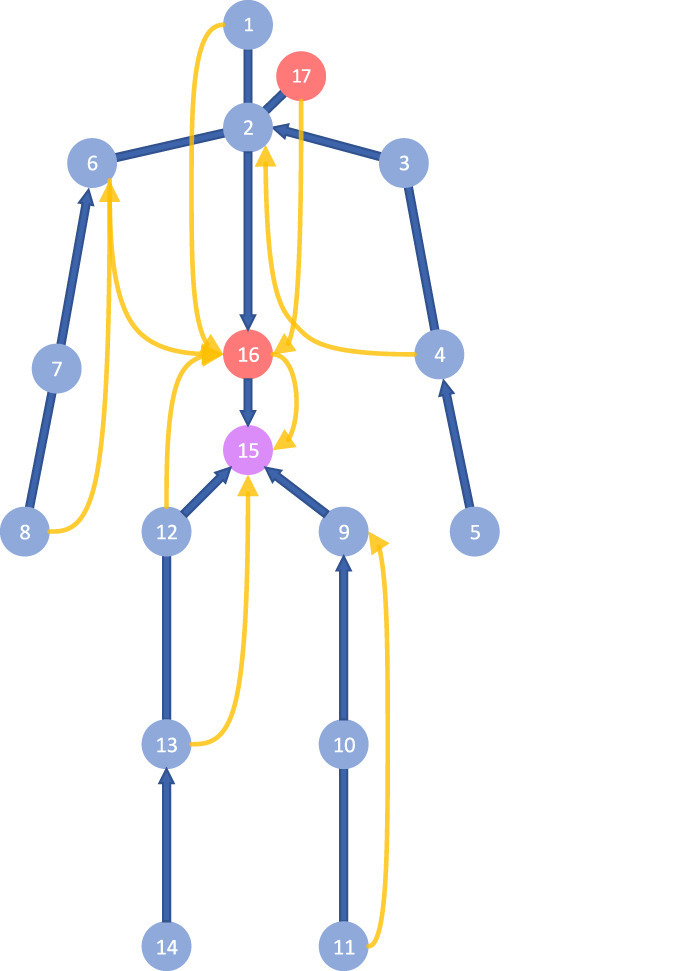
\includegraphics[scale=1.5]{images/3d_pose_estimation/skeleton_human_model.jpg}
    \caption[Μοντέλο Σκελετού]{\textsl{Μοντέλο Σκελετού ανθρώπινου σώματος}. Το σημείο κλειδί αναφοράς είναι το 15. Οι μπλε ακμές δείχνουν τους γονείς πρώτης τάξης του κάθε σημείου κλειδιού, ενώ οι κίτρινες ακμές τους γονείς δεύτερης τάξης (παραλείπονται κάποιοι για ευκρίνεια της εικόνας).}
    \label{fig:skeleton_model}
\end{figure}
    
\subsubsection{Μοντέλο σχήματος}
Το μοντέλο σχήματος αναπαριστά το ανθρώπινο σώμα ως ένα τριγωνικό πλέγμα καθορίζοντας έτσι πλήρως το σχήμα του σε οποιαδήποτε πόζα. Η μοντελοποίηση που χρησιμοποιείται στην πλειοψηφία των άρθρων εκτίμησης πόζας των τελευταίων χρόνων είναι το \engl{\textsl{skinned multi-person linear model} (SMPL)} \cite{smpl_paper}. Το μοντέλο \engl{SMPL}, το οποίο φαίνεται στο Σχήμα \ref{fig:smpl_model}, περιγράφει το ανθρώπινο δέρμα με 6890 κορυφές που σχηματίζουν το τριγωνικό πλέγμα. Οι κορυφές παραμετροποιούνται από τις παραμέτρους σχήματος $\vec{\beta}$ που καθορίζουν τις αναλογίες του σώματος, όπως το ύψος και τα κιλά, και τις παραμέτρους πόζας $\vec{\theta}$ που περιγράφουν τις περιστροφές των αρθρώσεων από μία πόζα αναφοράς.
    
\begin{figure}[h]
    \centering
    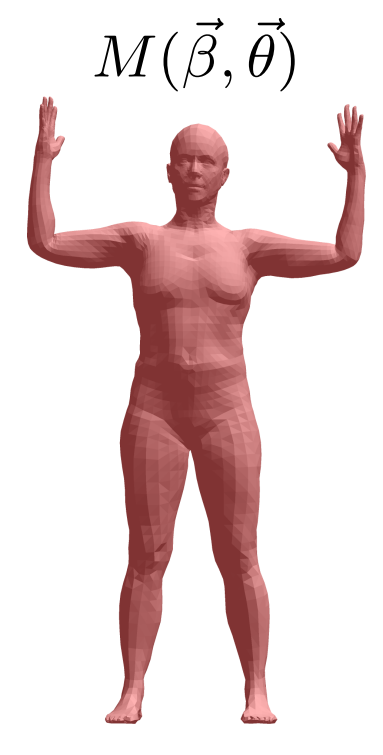
\includegraphics[scale=0.3]{images/3d_pose_estimation/smpl_model.png}
    \caption[Μοντελοποίηση \engl{SMPL}]{\textsl{Μοντελοποίηση \engl{SMPL}}. Το ανθρώπινο σώμα περιγράφεται από τις παραμέτρους σχήματος $\vec{\beta}$ και πόζας $\vec{\theta}$.}
    \label{fig:smpl_model}
\end{figure}
    
\subsubsection{Επιφανειακό μοντέλο}
Μία ακόμα πιο πρόσφατη μοντελοποίηση του ανθρώπινου σώματος για το πρόβλημα της εκτίμησης πόζας, αποτελεί το επιφανειακό μοντέλο. Αναπτύχθηκε με την εικασία ότι μία αραιή συσχέτιση της εικόνας με τα σημεία κλειδιά του ανθρώπινου σώματος δεν είναι αρκετή για να αντικατοπτρίσει τη πλήρη κατάσταση του. Τοιουτοτρόπως, στο άρθρο \cite{densepose_paper}, προτείνεται η επιφανειακή μοντελοποίηση, αποκαλούμενη \engl{DensePose}, όπου εγκαθιδρύεται μία πυκνή συσχέτιση των πίξελ της εικόνας με μία επιφανειακή αντιπροσώπευση του ανθρώπινου σώματος, όπως φαίνεται στο Σχήμα \ref{fig:densepose_correspondence} 

\begin{figure}[h]
    \centering
    \begin{subfigure}{.5\linewidth}
        \centering
        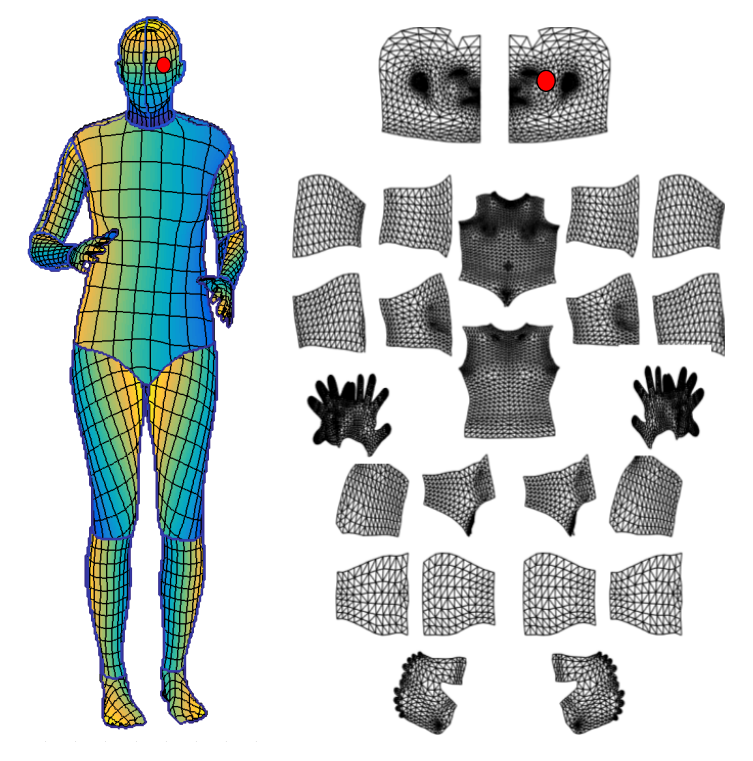
\includegraphics[width=.4\linewidth]{images/3d_pose_estimation/densepose_model.png}
    \end{subfigure}%
    \begin{subfigure}{.5\linewidth}
        \centering
        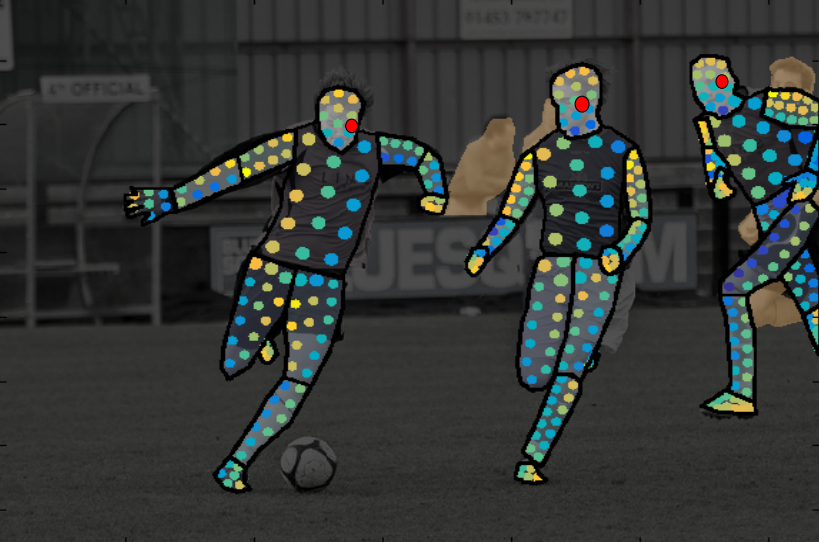
\includegraphics[width=.4\linewidth]{images/3d_pose_estimation/densepose_result_football.png}
    \end{subfigure}
    \caption[Μοντελοποίηση \engl{DensePose}]{\textsl{Μοντελοποίηση \engl{DensePose}}. Στα αριστερά φαίνεται η επιφανειακή τρισδιάστατη αναπαράσταση του ανθρώπινου σώματος. Αντιστοιχίζοντας τα σημεία της εικόνας δεξιά στην αριστερή επιφάνεια γίνεται δυνατή η εκτίμηση της πόζας.}
    \label{fig:densepose_correspondence}
\end{figure}

\subsection{Κατηγοριοποιήσεις λύσεων του προβλήματος εκτίμησης πόζας}

Για την επίλυση του προβλήματος εκτίμησης πόζας τα τελευταία χρόνια παρουσιάζονται ολοένα και περισσότερα άρθρα όπως φαίνεται στο Σχήμα \ref{fig:pose_estimation_papers}. Προφανώς, η κάθε προσέγγιση επίλυσης του προβλήματος έχει μοναδικά χαρακτηριστικά, ικανοποιώντας διαφορετικές απαιτήσεις, αλλά υπάρχουν κοινές κατευθυντήριες γραμμές πάνω στις οποίες κινούνται οι ερευνητές. Με αυτόν τον τρόπο, γίνεται δυνατή η κατηγοριοποίηση των λύσεων του προβλήματος ως προς τα διάφορα χαρακτηριστικά τους.

\begin{figure}[h]
    \centering
    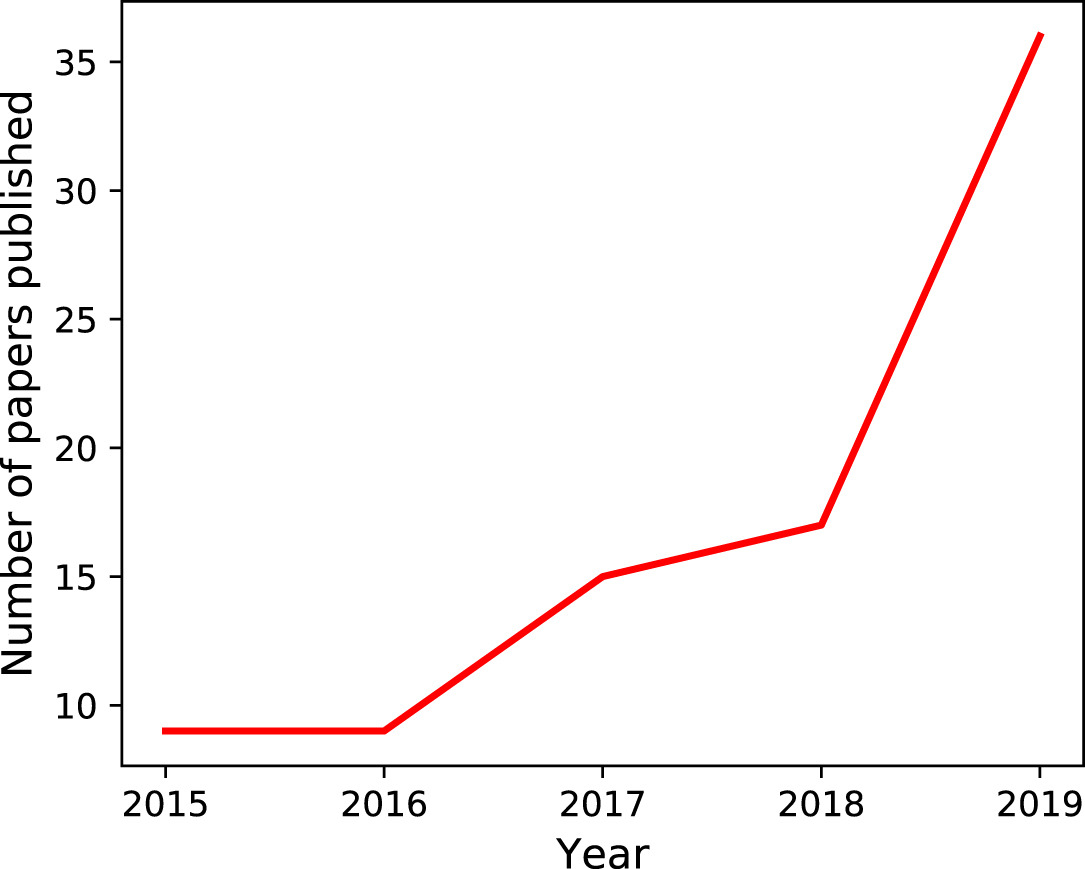
\includegraphics[scale=1.5]{images/3d_pose_estimation/pose_estimation_papers_per_year.jpg}
    \caption[Άρθρα εκτίμησης πόζας ανά χρόνο]{Αριθμός άρθρων εκτίμησης ανθρώπινης πόζας (κατακόρυφος άξονας) ανά χρόνο (οριζόντιος άξονας)}
    \label{fig:pose_estimation_papers}
\end{figure}

Η γενικότερη κατηγοριοποίηση αφορά την μορφή της εισόδου του μοντέλου μηχανικής μάθησης. Με άλλα λόγια, το μοντέλο μπορεί να χρησιμοποιεί για είσοδο μόνο μία εικόνα ή πολλαπλές εικόνες από διαφορετικές οπτικές (της ίδιας χρονικής στιγμής). Αντίθετα, για την αξιοποίηση της χρονικής πληροφορίας, μπορεί να χρησιμοποιηθεί ως είσοδος αλληλουχίες εικόνων, είτε μεμονωμένων είτε από διαφορετικές οπτικές. Προφανώς, οι πιο περίπλοκες είσοδοι απαιτούν περισσότερους πόρους τόσο για την ανάκτηση των εικόνων όσο και για την επεξεργασία τους, μειώνοντας ωστόσο τις ασάφειες του προβλήματος.

Επιπλέον, οι μεθοδολογίες της εκτίμησης πόζας μπορούν να διαχωριστούν ανάλογα με την ικανότητα τους στην πρόβλεψη πόζας ενός ή περισσότερων ανθρώπων. Στην πρώτη περίπτωση, ορίζεται η πρόβλεψη της πόζας μόνο για έναν άνθρωπο μέσα στην εικόνα και είναι σαφώς η απλούστερη. Στην περίπτωση εκτίμησης πόζας περισσότερων ανθρώπων το πρόβλημα δυσχεραίνεται λόγω του πολύ μεγαλύτερου χώρου καταστάσεων, της απόκρυψης ή και σύγχυσης των σημείων κλειδιών και της αναγκαιότητας διαφοροποίησης τους.

Τοιουτοτρόπως, συγκεκριμένα για το πρόβλημα εκτίμησης πόζας πολλαπλών ανθρώπων, διακρίνουμε την κατηγοριοποίηση με βάση τον τρόπο ομαδοποίησης των σημείων κλειδιών στους ανθρώπους στους οποίους ανήκουν. Οι δύο κύριες προσεγγίσεις είναι η \textsl{από κάτω προς τα πάνω} και η \textsl{από πάνω προς τα κάτω}.

\begin{itemize}
    \item \textsl{Aπό κάτω προς τα πάνω}: Το μοντέλο ανιχνεύει κάθε εμφάνιση ενός συγκεκριμένου σημείου κλειδιού (όπως όλα τα αριστερά χέρια) σε μία εικόνα και στην συνέχεια προσπαθεί να ομαδοποιήσει τα σημεία κλειδιά με βάση τους ανθρώπους στους οποίους ανήκουν. 
    \item \textsl{Aπό πάνω προς τα κάτω}: Αντίθετα, σε αυτή την μέθοδο, το μοντέλο αρχικά χρησιμοποιεί έναν ανιχνευτή αντικειμένων, καθορίζοντας έτσι ένα πλαίσιο οριοθέτησης γύρω από κάθε άνθρωπο, και έπειτα εκτιμά την θέση των σημείων κλειδιών του κάθε ανθρώπου εσωτερικά σε κάθε περικομμένη περιοχή.
\end{itemize}

Μία άλλη πιθανή κατηγοριοποίηση σχετίζεται με τα χρησιμοποιούμενα στάδια προβλέψεων έως ότου προκύψει η τελική εκτίμηση πόζας. Αναλυτικότερα, θα αναλύσουμε τις μεθόδους από τρεις κατηγορίες: εκτίμηση τρισδιάστατης πόζας απευθείας από εικόνες, ανύψωση από δισδιάστατες σε τρισδιάστατες προβλέψεις και μεθόδους βασισμένες στο μοντέλο \engl{SMPL}. 

\subsubsection{Εκτίμηση πόζας απευθείας από εικόνες}

Η πιο άμεση μεθοδολογία για την εκτίμηση της τρισδιάστατης πόζας είναι ο σχεδιασμός συνεχόμενων δικτύων για την πρόβλεψη των \engl{3D} συντεταγμένων των σημείων κλειδιών ή αρθρώσεων. Οι μέθοδοι της απευθείας εκτίμησης από εικόνες μπορούν να διαχωριστούν περαιτέρω σε δύο κλάσεις: μέθοδοι βασισμένες στον εντοπισμό και μέθοδοι βασισμένες στην παλινδρόμηση. Αξίζει να σημειωθεί ότι έχουν γίνει προσπάθειες για ενοποίηση των δύο αυτών προσεγγίσεων.

Οι μέθοδοι βασισμένες στον εντοπισμό προβλέπουν έναν πιθανοτικό θερμικό χάρτη για κάθε σημείο κλειδί και παίρνοντας την μέγιστη πιθανότητα του χάρτη καθορίζουν την θέση του σημείου κλειδιού. Για παράδειγμα στο \cite{pavlakos_paper} αναπαριστάται ο τρισδιάστατος χώρος σε έναν όγκο και εκπαιδεύεται ένα μοντέλο Συνελικτικού Νευρωνικού Δικτύου (\engl{\textsl{Convolutional Neural Network, CNN}} στο καθεξής) ώστε να προβλέπονται οι ογκομετρικοί πιθανοτικοί θερμικοί χάρτες για κάθε σημείο κλειδί, όπως φαίνεται στο Σχήμα \ref{fig:pavlakos_architecture}. Παρόμοιες μέθοδοι βασίζονται σε επιπλέον βήματα για την μετατροπή των θερμικών χαρτών στην τελική εκτίμηση των θέσεων των σημείων κλειδιών, συνήθως παίρνοντας την μέγιστη πιθανότητα του χάρτη, δηλαδή εφαρμόζοντας την συνάρτηση \engl{argmax} (βλ. στο παράρτημα τον ορισμό \ref{definition:argmax} ). Βέβαια, η διαδικασία αυτή δεν είναι διαφορίσιμη, αποτελώντας τροχοπέδη στον μηχανισμό εκμάθησης των νευρωνικών δικτύων. Ταυτόχρονα, η ακρίβεια των προβλεπόμενων σημείων κλειδιών είναι ανάλογη της διακριτότητας των θερμικών χαρτών ο οποίοι έχουν εγγενή αδυναμία στη χωρική γενίκευση. Για την αύξηση της ακρίβειας των προβλέψεων, οι παραγόμενοι θερμικοί χάρτες απαιτούν αύξηση της χωρικής διακριτότητας, αυξάνοντας όμως τετραγωνικά τις απαιτήσεις σε υπολογιστική ισχύ και κατανάλωση μνήμης.

\begin{figure}[h]
    \centering
    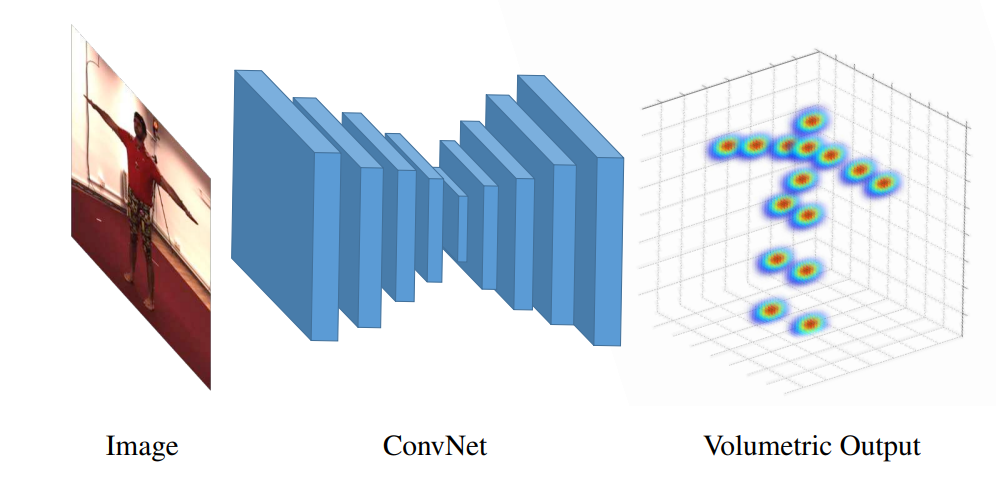
\includegraphics[scale=0.4]{images/3d_pose_estimation/pavlakos_architecture.png}
    \caption[Μέθοδος εκτίμησης πόζας βασισμένη στον εντοπισμό]{\textsl{Μέθοδος εκτίμησης πόζας βασισμένη στον εντοπισμό}. Η εικόνα ως είσοδος περνάει από την αρχιτεκτονική του \engl{CNN} και παράγει πιθανοτικούς χάρτες για κάθε σημείο κλειδί στον \engl{3D} χώρο.}
    \label{fig:pavlakos_architecture}
\end{figure}

Από την άλλη μεριά, το πρόβλημα εκτίμησης πόζας μπορεί να θεωρηθεί διαισθητικά ως ένα πρόβλημα παλινδρόμησης,  όπου εκτιμούνται οι συντεταγμένες θέσεων των σημείων κλειδιών ως προς την θέση ενός σημείου κλειδιού αναφοράς\footnote{Στο μοντέλο σκελετού \engl{\textsl{SMPL}}, για παράδειγμα, το σημείο αναφοράς, σημείο με δείκτη (\engl{\textsl{index}}) 0, είναι η λεκάνη}. Σε αυτή την προσέγγιση, γίνεται εμφανής η καταλληλότητα επιλογής των \textsl{μοντέλων σκελετού} ή παρεμφερή μοντελοποιήσεις για την αναπαράσταση του ανθρώπινου σώματος. Για παράδειγμα, για να ενσωματώσουν προηγούμενη γνώση για την δομή του ανθρώπινου σώματος, στο \cite{kinematic_pose_regression_paper}, εισάγουν ένα \textsl{κινηματικό μοντέλο σκελετού}, αποτελούμενο από αρθρώσεις και κόκαλα, τα οποία κόκαλα έχουν σταθερό μήκος και μπορούν να περιστραφούν γύρω από τις αρθρώσεις. Εντούτοις, το σταθερό μήκος των κοκάλων δεν ανταποκρίνεται επαρκώς στη μεταβλητότητα του ανθρώπινου σκελετού, γεγονός που υποβαθμίζει την ικανότητα γενικοποίησης του μοντέλου. Από την άλλη μεριά, στο \cite{composition_human_pose_regression} υποθέτουν ότι στην εκτίμηση πόζας είναι πιο λογική η εκτίμηση της θέσεως των κοκάλων αντί για τις αρθρώσεις διότι η αναπαράσταση των κοκάλων καθιστά ευκολότερη την εκμάθηση του \textsl{μοντέλου βαθιάς μάθησης} και αντικατοπτρίζουν καλύτερα τους γεωμετρικούς περιορισμούς του ανθρώπινου σκελετού. Φυσικά, αυτή η προσέγγιση απαιτεί την μετατροπή των δεδομένων εκπαίδευσης στην σχετική μορφή αναπαράστασης τις θέσεις των κοκάλων. 

Εν κατακλείδι, οι μέθοδοι εντοπισμού με θερμικούς χάρτες, αν και πιο αποδοτικοί από τις μεθόδους παλινδρόμησης, έχουν κάποια μειονεκτήματα. Η διαδικασία επιλογής της μέγιστης πιθανότητας δεν είναι διαφορίσιμη και δεν επιτρέπει την από άκρη σε άκρη εκμάθηση του μοντέλου, σε αντίθεση με τις μεθόδους παλινδρόμησης όπου αυτή η εκμάθηση είναι εφικτή.

Προς αντιμετώπιση των προαναφερθέντων προβλημάτων έχουν γίνει προσπάθειες συνδυασμού των δύο παραπάνω μεθόδων. Για παράδειγμα, στο άρθρο \cite{human_pose_regression_paper}, προτείνεται η χρήση της συνάρτησης \engl{soft-argmax} (αναλυτικότερα βλ. ορισμό \ref{definition:soft-argmax}) για την μετατροπή των χαρτών χαρακτηριστικών (\engl{feature maps}), ή των θερμικών χαρτών, σε συντεταγμένες των σημείων κλειδιών, έχοντας ως αποτέλεσμα ένα πλήρως διαφορίσιμο σύστημα. Με παρόμοια λογική με την συνάρτηση \engl{soft-argmax}, στο άρθρο \cite{numerical_coordinate_regression_paper}, εισάγουν ένα καινούργιο επίπεδο, αποκαλούμενο διαφορίσιμη χωρική σε αριθμητική μετατροπή (\engl{differentiable spatial to numerical transform, DSNT}), για να διατηρήσουν την από από άκρη σε άκρη δυνατότητα εκμάθησης του μοντέλου και ταυτόχρονα βελτιώνοντας την ικανότητα γενικοποίησης του. 

\subsubsection{Ανύψωση προβλέψεων από \engl{2D} σε \engl{3D} }

Εμπνευσμένοι από την ραγδαία εξέλιξη των αλγορίθμων για εκτίμηση της \engl{2D} πόζας, αρκετοί ερευνητές προσπάθησαν να χρησιμοποιήσουν τα αποτελέσματα της \engl{2D} εκτίμησης πόζας για να βελτιώσουν την ικανότητα γενικοποίησης σε δεδομένα αποκτημένα υπό καθημερινές συνθήκες. 

Χαρακτηριστικό παράδειγμα αποτελεί η έρευνα στο \cite{simple_baseline_pose_estimation} όπου προτείνεται μία αρχιτεκτονική, όπως φαίνεται στο Σχήμα \ref{fig:simple_baseline}, επικεντρωμένη στην ανύψωση της \engl{2D} πόζας σε \engl{3D} με ένα απλό αλλά αποδοτικό νευρωνικό δίκτυο, εμφυσώντας ενδιαφέρον για περαιτέρω έρευνα στην ανύψωση της \engl{2D} πόζας στον \engl{3D} χώρο.

\begin{figure}[h]
    \centering
    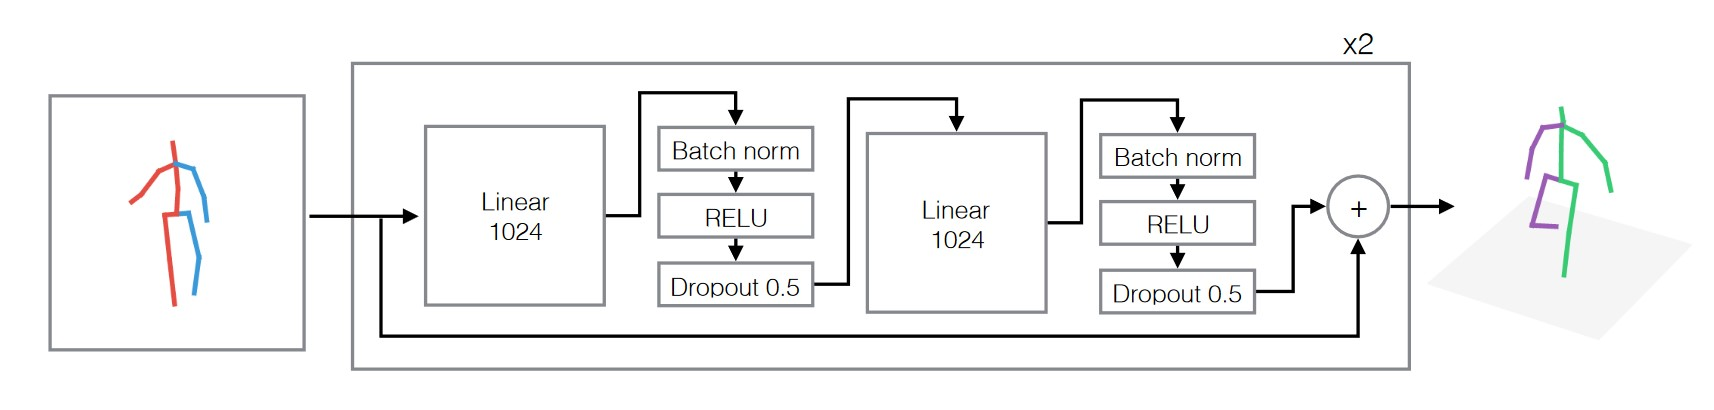
\includegraphics[scale=0.5]{images/3d_pose_estimation/simple_baseline_architecture.jpg}
    \caption[Αρχιτεκτονική \engl{simple baseline} για την εκτίμηση πόζας]{Αρχιτεκτονική \engl{simple baseline} για την εκτίμηση πόζας. Ακρογωνιαίος λίθος του νευρωνικού αποτελεί ένα γραμμικό επίπεδο, ακολουθούμενο από ένα επίπεδο κανονικοποίησης παρτίδας (\engl{batch normalization}), ένα επίπεδο ενεργοποίησης με συνάρτηση \engl{ReLU} (βλ. παράρτημα \ref{definition:relu}) και ένα επίπεδο εγκατάλειψης μονάδων εισόδου (\engl{dropout}). Η είσοδος του συστήματος είναι ένας πίνακας με τις \engl{2D} θέσεις των σημείων κλειδιών και η έξοδος είναι οι θέσεις των σημείων κλειδιών σε \engl{3D} συντεταγμένες.}
    \label{fig:simple_baseline}
\end{figure}

Για την αντιμετώπιση της δυσκολίας παραγωγής και σχολιασμού εξολοκλήρου \engl{3D} συνόλων δεδομένων σε διάφορες έρευνες χρησιμοποιούνται επιπλέον πληροφορίες ως ενδιάμεση επίβλεψη του συστήματος. Ένα είδος πληροφορίας που χρησιμοποιείται συχνά είναι η προβολή της προβλεπόμενης \engl{3D} πόζας στον \engl{2D} χώρο της εικόνας. Για παράδειγμα στο \cite{lifting_from_the_deep}, αρχικά εκτιμάται η \engl{2D} πόζα η οποία χρησιμοποιείται για την εκτίμηση της \engl{3D} πόζας. Έπειτα, οι προβλέψεις της \engl{3D} πόζας προβάλλονται στον \engl{2D} χώρο, συνδυάζονται με τις αρχικές \engl{2D} προβλέψεις και τέλος συγκρίνονται με τους \engl{2D} σχολιασμούς του συνόλου δεδομένων (όπως φαίνεται στο Σχήμα \ref{fig:lifting_from_the_deep_architecture}), εκπαιδεύοντας έτσι το σύστημα. Αξίζει να σημειωθεί ότι στο στάδιο ανύψωσης των \engl{2D} προβλέψεων σε \engl{3D} ενσωματώνεται ένα επιπλέον επίπεδο στο \engl{CNN} όπου αναπαριστώνται οι \engl{3D} γεωμετρικοί περιορισμοί του σώματος, ενός \textsl{μοντέλου σκελετού} (όπως αναπτύχθηκε στην ενότητα \ref{section:skeleton_model}), εξασφαλίζοντας ότι οι προβλεπόμενες πόζες βρίσκονται στον χώρο των επιτρεπόμενων εκ φύσεως ποζών. 

\begin{figure}[h]
    \centering
    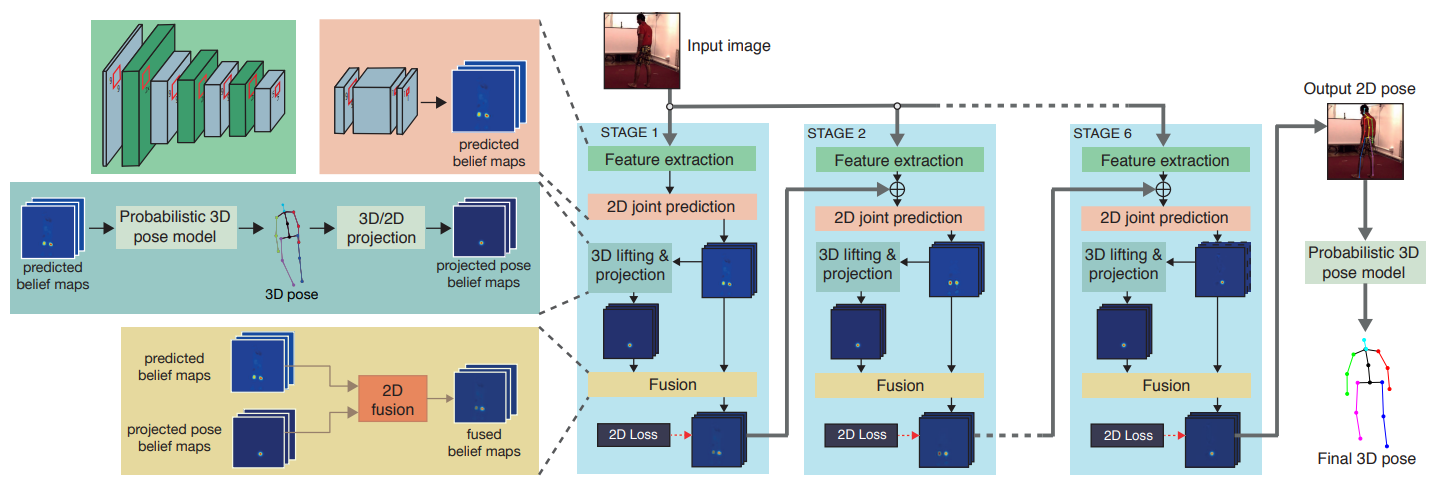
\includegraphics[scale=0.3]{images/3d_pose_estimation/lifting_from_the_deep_architecture.png}
    \caption[\engl{Lifting from the deep}: Παράδειγμα αρχιτεκτονικής ανύψωσης \engl{2D} σε \engl{3D}]{\textsl{\engl{Lifting from the deep}: Παράδειγμα αρχιτεκτονικής ανύψωσης \engl{2D} σε \engl{3D}}. Κάθε στάδιο παράγει ως έξοδο ένα σύνολο \engl{2D} πιθανοτικών χαρτών για κάθε σημείο κλειδί, οι οποίοι μαζί με την αρχική εικόνα αποτελούν την είσοδο του επόμενο σταδίου. Κάθε στάδιο μαθαίνει να συνδυάζει τους πιθανοτικούς χάρτες της \engl{2D} εκτίμησης πόζας με τους προβαλλόμενους χάρτες από την \engl{3D} εκτίμηση πόζας.}
    \label{fig:lifting_from_the_deep_architecture}
\end{figure}

Αντίστοιχα για την αποφυγή σχολιασμού των \engl{3D} συνόλων δεδομένων, στο \cite{ordinal_depth_supervision}, προτείνεται μία εναλλακτική, πιο ασθενής μέθοδος επίβλεψης του συστήματος. Πιο συγκεκριμένα, για την επίβλεψη χρησιμοποιούνται οι ήδη υπάρχοντες σχολιασμοί των \engl{2D} σημείων κλειδιών σε συνδυασμό με τις σχέσεις βάθους (πιο κοντά - πιο μακριά) των σημείων κλειδιών, όπως φαίνεται στο Σχήμα \ref{fig:ordinal_depth_architecture}. Μάλιστα, παρουσιάζεται η ευελιξία αυτής της μεθόδου επίβλεψης, ενσωματώνοντάς την σε διαφορετικές διαρρυθμίσεις νευρωνικών δικτύων όπου επιτυγχάνονται ανταγωνιστικά αποτελέσματα με την επίβλεψη με πραγματικούς \engl{3D} σχολιασμούς του συνόλου δεδομένων.
 
 \begin{figure}[h]
    \centering
    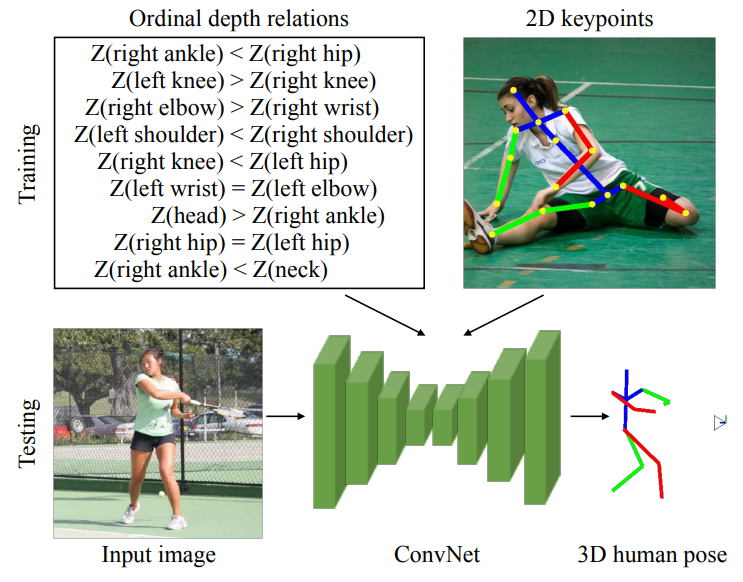
\includegraphics[scale=0.5]{images/3d_pose_estimation/ordinal_depth_architecture.png}
    \caption[\engl{Ordinal Depth Supervision}: Παράδειγμα αρχιτεκτονικής ανύψωσης \engl{2D} σε \engl{3D}]{\textsl{\engl{Ordinal Depth Supervision}: Παράδειγμα αρχιτεκτονικής ανύψωσης \engl{2D} σε \engl{3D}}. Όταν εκλείπουν οι \engl{3D} σχολιασμοί του συνόλου δεδομένου, μπορούν να χρησιμοποιηθούν οι \engl{2D} σχολιασμοί των σημείων κλειδιών σε συνδυασμό με τις σχέσεις βάθους των σημείων κλειδιών.}
    \label{fig:ordinal_depth_architecture}
\end{figure}

\subsubsection{Μέθοδοι βασισμένες στο μοντέλο σχήματος \engl{SMPL}}



%-----------------------------------------------------
\subsection{Αρχιτεκτονικές μοντέλων μηχανικής μάθησης}

Οι αρχιτεκτονικές \textsl{βαθιάς μηχανικής μάθησης} για την εκτίμηση πόζας παίρνουν πολλαπλές μορφές. Οι περισσότερες χρησιμοποιούν αρχικά ένα κωδικοποιητή ο οποίος δέχεται ως είσοδο την εικόνα ή πλαίσια αυτής και εξάγει κάποια χαρακτηριστικά (\engl{\textsl{features}}). Το επόμενο βήμα, εξαρτάται κατά κόρον από την εκάστοτε υλοποίηση.

Η πιο απλή τεχνική χρησιμοποιεί έναν \textsl{παλινδρομητή} (\textsl{\engl{regressor}}), ο οποίος δέχεται ως είσοδο τα εξαγόμενα χαρακτηριστικά από τον κωδικοποιητή και παράγει τις τελικές εκτιμήσεις των τρισδιάστατων συντεταγμένων για κάθε σημείο κλειδί. 

Μία ελαφρώς πιο περίπλοκη τεχνική χρησιμοποιεί αρχιτεκτονική κωδικοποιητή - αποκωδικοποιητή. Τα εξαγόμενα χαρακτηριστικά του κωδικοποιητή εισάγονται σε έναν αποκωδικοποιητή ο οποίος παράγει θερμικούς χάρτες αναπαριστώντας την πιθανότητα ενός σημείου κλειδιού να βρίσκεται σε κάποια περιοχή της εικόνας ή του χώρου.

Οι δύο προαναφερθείσες τεχνικές μπορούν να εφαρμοστούν στην εκτίμηση τόσο της δισδιάστατης όσο και της τρισδιάστατης πόζας. Στην περίπτωση όμως της τρισδιάστατης εκτίμησης πόζας υφίσταται μία ακόμα επιλογή. Αντί για την εκτίμηση των συντεταγμένων των σημείων κλειδιών, είναι πιθανό να εκτιμηθούν οι τιμές των παραμέτρων κάθε βαθμού ελευθερίας όλων των αρθρώσεων και στην συνέχεια να εφαρμοστούν οι μετασχηματισμοί στις αρθρώσεις από μία πόζα αναφοράς.

Και στις δύο προσεγγίσεις, οι αρχιτεκτονικές \textsl{βαθιάς μηχανικής μάθησης} κατάλληλες για ανάλυση της εικόνας έχουν ως ακρογωνιαίο λίθο κάποια παραλλαγή ενός \textsl{Συνελικτικού Νευρωνικού Δικτύου} (\engl{\textsl{Convolutional Neural Network, CNN}}).



%%% Εργαλεία %%%
\chapter{Εργαλεία}
\section{\texorpdfstring{\engl{Kivy}}{Kivy}}

\begin{figure}[h]
    \centering
    
\includegraphics[scale=0.5]{images/kivy_logo.png}
    \caption{\engl{Kivy}}
\end{figure}

Το \engl{Kivy\footnote{\href{https://kivy.org/}{https://kivy.org/}}} είναι μια βιβλιοθήκη ανοιχτού κώδικα της \engl{Python} για την γρήγορη ανάπτυξη εφαρμογών που χρησιμοποιούν γραφικά για υλοποίηση καινοτόμων διεπαφών χρηστών. Επιλέξαμε την εν λόγω βιβλιοθήκη για την υλοποίηση της διεπαφής του καθρέφτη επειδή είναι:
\begin{itemize}
    \item \textbf{\engl{Cross Platform}:} Το \engl{Kivy} τρέχει σε διαφορετικά λειτουργικά συστήματα και πλατφόρμες όπως \engl{Windows, Linux, Android, OS X, Raspberry Pi} με τον ίδιο κώδικα.
    \item \textbf{\engl{GPU Accelerated}:} Η μηχανή γραφικών έχει υλοποιηθεί πάνω στην \engl{OpenGL ES 2} χρησιμοποιώντας μια σύγχρονη και γρήγορη γραμμή γραφικών.
    \item \textbf{Εύκολη στη Χρήση:} Περιλαμβάνει μια ευρεία γκάμα έτοιμων \engl{widgets} ενώ χρησιμοποιεί μια απλή ενδιάμεση γλώσσα (\engl{kv}) για τον εύκολο σχεδιασμό \engl{widget} από τον χρήστη.
\end{itemize}

\subsection{Αρχιτεκτονική του \texorpdfstring{\engl{Kivy}}{Kivy}}
Το \engl{Kivy} αποτελείται από πολλά δομικά κομμάτια όπως φαίνεται στο Σχήμα \ref{fig:kivy_arch}. Κάποια βασικά από αυτά τα δομικά κομμάτια περιγράφονται στη συνέχεια \cite{kivy}.

\begin{figure}[ht]
    \centering
    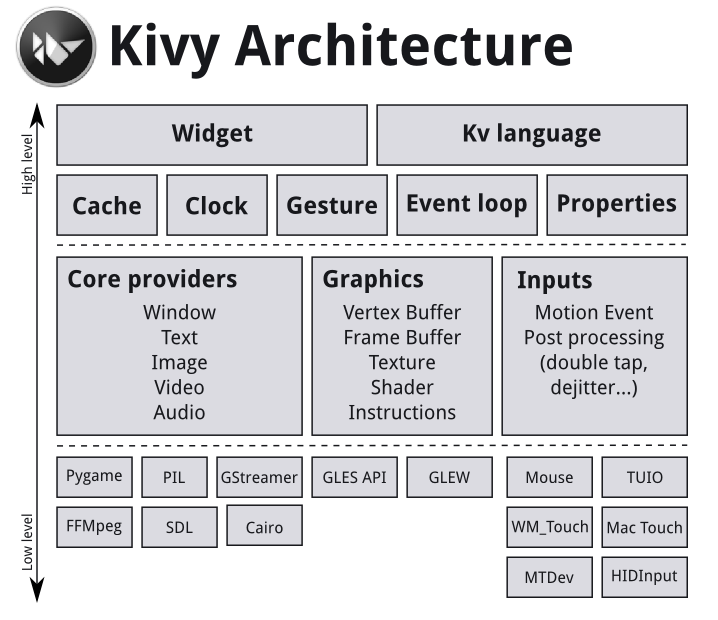
\includegraphics[scale=0.5]{images/kivy_architecture.png}
    \caption{Αρχιτεκτονική της βιβλιοθήκης \engl{Kivy}}
    \label{fig:kivy_arch}
\end{figure}

\subsubsection{\engl{Core} και \engl{Input Providers}}
Ένας \engl{Core Provider} είναι ένα κομμάτι κώδικα που λειτουργεί ως διαμεσολαβητής ανάμεσα στο ΛΣ και το \engl{Kivy}. Η βασική ιδέα είναι να χωριστούν εργασίες όπως το άνοιγμα ενός παραθύρου, η εμφάνιση μια εικόνας ή κειμένου, η αναπαραγωγή ήχου κτλ. έτσι ώστε το \engl{API} να είναι εύχρηστο και επεκτάσιμο. Το βασικότερο πλεονέκτημα όμως είναι ότι με αυτόν τον τρόπο επιτρέπεται να χρησιμοποιηθούν συγκεκριμένοι \engl{providers} ανάλογα με τα σενάρια χρήσης της εφαρμογής. Για παράδειγμα, τα \engl{OS X, Linux} και \engl{Windows} χρησιμοποιούν διαφορετικούς \engl{providers} για τις παραπάνω εργασίες. Με τη χρήση εξειδικευμένων \engl{providers} για κάθε πλατφόρμα είναι εφικτή η πλήρης αξιοποίηση του ΛΣ με αποδοτικό τρόπο, ενώ είναι εφικτή η μεταφορά της εφαρμογής σε άλλες πλατφόρμες αρκετά εύκολα.

Με αντίστοιχο τρόπο δουλεύουν και οι \engl{providers} εισόδων. Αν κάποιος θέλει να υποστηρίξει μια νέα συσκευή εισόδου χρειάζεται απλά να γράψει μία κλάση η οποία διαβάζει τα δεδομένα της συγκεκριμένης συσκευής και τα μεταφράζει και γεγονότα του \engl{Kivy (Kivy Events)}.

\subsubsection{Γραφικά}
Το γραφικό \engl{API} του \engl{Kivy} είναι μια αφαιρετικότητα της \engl{OpenGL}. Στο χαμηλότερο επίπεδο το \engl{Kivy} δίνει \engl{hardware accelerated} εντολές σχεδιασμού χρησιμοποιώντας \engl{OpenGL}. Αλλά επειδή το να γράφει κανείς σε \engl{OpenGL} είναι επίπονο, ειδικά για τους νέους χρήστες, είναι εφικτό να σχεδιαστού γραφικά χρησιμοποιώντας μεταφορικές εντολές (\engl{Canvas, Rectangle} κτλ.) που δεν υπάρχουν στην \engl{OpenGL}.  

\subsubsection{Πυρήνας}
Ο κώδικας του πακέτου του πυρήνα παρέχει συχνά χρησιμοποιούμενα χαρακτηριστικά όπως:
\begin{itemize}
    \item Το \textbf{ρολόι} που χρησιμοποιείται για να προγραμματιστούν χρονικά γεγονότα.
    \item Την \textbf{\engl{cache}} σε περίπτωση που κάποιος θέλει να αποθηκεύσει κάτι που χρησιμοποιείται συχνά.
    \item Την \textbf{αναγνώριση χειρονομίας} για αποθήκευση και ανίχνευση διαφόρων σχημάτων, όπως κύκλοι, ενώ μπορεί να εκπαιδευτεί για σχήματα που καθορίζει ο χρήστης.
    \item Την \textbf{γλώσσα \engl{Kivy}} η οποία χρησιμοποιείται για να περιγραφούν με ευκολία και αποδοτικότητα οι διεπαφές χρηστών
    \item Τις \textbf{ιδιότητες} οι οποίες είναι κλάσεις που συνδέουν τον κώδικα ενός \engl{widget} με την περιγραφή της διεπαφής του χρήστη.
\end{itemize}

\subsubsection{\engl{UIX}}
Το συγκεκριμένο πακέτο περιέχει τα πιο συχνά χρησιμοποιούμενα \engl{widgets} και \engl{layouts} για την γρήγορη ανάπτυξη μια διεπαφής χρήστη.
\begin{itemize}
    \item Τα \textbf{\engl{widgets}} είναι στοιχεία διεπαφής τα οποία εισάγονται στο πρόγραμμα και παρέχουν κάποια λειτουργία όπως πχ. κουμπιά, λίστες, επιγραφές κ.α.
    \item Τα \textbf{\engl{layouts}} χρησιμοποιούνται για την διάταξη των \engl{widgets}.
\end{itemize}

\section{\texorpdfstring{\engl{Wit.ai}}{Wit.ai}}
\begin{figure}[h]
    \centering
    
\includegraphics[scale=0.6]{images/wit_logo.png}
    \caption{\engl{Wit.ai}}
\end{figure}
Το \engl{Wit\footnote{\href{https://wit.ai/}{https://wit.ai/}}} είναι ένα \engl{framework} ανοιχτού κώδικα που επιτρέπει του χρήστες να αλληλεπιδρούν με την εφαρμογή μέσως φωνής και βασίζεται στη χρήση ισχυρού \engl{NLP (Natural Language Processing)}. Η λειτουργία του \engl{Wit} μπορεί να χωριστεί σε 2 βασικές κατηγορίες, την \textbf{ταξινόμηση πρόθεσης} (\engl{intent classification}) και την \textbf{εξαγωγή οντοτήτων} (\engl{entity extraction}).

Το \engl{Wit} επιτρέπει μια εφαρμογή να καταλάβει τους χρήστες. Αρχικά μπορεί ο προγραμματιστής μέσω της πλατφόρμας να δώσει κάποιες \textbf{εκφράσεις} (\engl{utterances}) ως παραδείγματα στις οποίες ορίζει την πρόθεση και τις οντότητες που περιέχουν προκειμένου να εκπαιδευτεί το μοντέλο. Για παράδειγμα μπορούμε να δώσουμε ως έκφραση την παρακάτω πρόταση:

\enquote{\engl{What's the temperature?}}

\noindentκαι να ορίσουμε ως πρόθεση \texttt{\engl{temperature\_get}}. Με αυτόν τον τρόπο μαθαίνουμε στο \engl{Wit} ότι με αυτήν την έκφραση ο χρήστης δηλώνει την πρόθεσή του να μάθει την θερμοκρασία. Όταν επομένως ρωτήσει ο χρήστης το \engl{Wit} για την θερμοκρασία (είτε με την παραπάνω έκφραση είτε με μια παρόμοια όπως \enquote{\engl{I would like to know the temperature}}) το \engl{Wit} θα προσπαθήσει να προβλέψει την πρόθεση του χρήστη δίνοντας και μία μετρική της σιγουριάς (\engl{confidence}) από 0 έως 1. Όσα περισσότερα παραδείγματα δώσουμε τόσο μεγαλύτερη γίνεται η σιγουριά και η ικανότητα του \engl{Wit} για την πρόβλεψη της πρόθεσης.

Έστω ότι δίνεται ως είσοδος στο \engl{Wit} η έκφραση \enquote{\engl{set the temperature to 70 degrees}}. Η απάντηση που θα δοθεί θα έχει την εξής μορφή:

\begin{otherlanguage}{english}
\begin{lstlisting}[language=Python]
{
    "text": "set the temperature to 70 degrees",
    "intents": [
        {
            "id": "226127658493500",
            "name": "temperature_get",
            "confidence": 0.9953
        }
    ],
    "entities": [],
    "traits": []
}
\end{lstlisting}
\end{otherlanguage}

Η απάντηση όμως δεν είναι ικανοποιητική αφού η πρόθεση του χρήστη είναι να αλλάξει η θερμοκρασία και όχι να πάρει την θερμοκρασία κάτι που είναι λογικό αφού το \engl{Wit} καταλαβαίνει μόνο μία πρόθεση. Μέσω της πλατφόρμας όμως είναι εύκολο να αλλάξουμε την πρόθεση μιας ήδη δοσμένης έκφρασης και να ξαναεκπαιδευτεί το μοντέλο θέτοντας αυτή τη φορά την πρόθεση \texttt{\engl{temperature\_set}}. Δίνεται επίσης η επιλογή να ορίστει ένα κατώφλι σιγουριάς έτσι ώστε να μην επιστρέφονται προθέσεις κάτω από αυτό το όριο.

Στο παραπάνω παράδειγμα, θέλουμε να αποσπάσουμε μαζί με την πρόθεση και το νούμερο της επιθυμητής θερμοκρασίας. Κάτι τέτοιο είναι εύκολο μέσω της πλατφόρμας όπου μπορούμε να ορίσουμε το \texttt{\engl{70 degrees}} να είναι μια οντότητα (πχ \texttt{\engl{temperature\_degrees}}). Έτσι στην απάντηση που θα λάβει η εφαρμογή από το \engl{Wit} θα μπορεί να εξάγει και τον αριθμό των βαθμών έτσι ώστε να προβεί στην κατάλληλη πράξη για να θέσει την θερμοκρασία στην επιθυμητή τιμή.

Η επιλογή του \engl{Wit} έγινε ανάμεσα σε αρκετά αντίστοιχα εργαλεία ανοιχτού κώδικα που υπάρχουν διαθέσιμα όπως το \engl{spaCy\footnote{\href{https://spacy.io/}{https://spacy.io/}}} ή το \engl{Rasa\footnote{\href{https://rasa.com/open-source/}{https://rasa.com/open-source/}}}. Ο βασικός λόγος επιλογής του \engl{Wit} είναι η ευκολία εκπαίδευσης και προσαρμογής του μέσω της πλατφόρμας. Επίσης, η ενσωμάτωση στην εφαρμογή ήταν πολύ εύκολη με τη χρήση της βιβλιοθήκης\footnote{\engl{\href{https://github.com/wit-ai/pywit}{https://github.com/wit-ai/pywit}}} που παρέχει το \engl{Wit} για \engl{Python}, το \engl{documentation} ήταν αρκετά κατατοπιστικό και η δομή των δεδομένων στην απάντηση του \engl{Wit} το έκαναν εύκολο στην χρήση. Τέλος, είναι δυνατό κανείς να κατεβάσει τα δεδομένα ενός ήδη εκπαιδευμένου μοντέλου, και να δημιουργήσει ένα με βάση αυτά όποτε και να μπορεί στη συνέχει να το επεκτείνει με δικές του εντολές και να το προσαρμόσει στις ανάγκες των δικών του εφαρμογών, βοηθώντας κατά αυτόν τον τρόπο στην επεκτασιμότητα της διεπαφής του καθρέφτη.

\section{Χειρισμός Φωνής}
Για την αλληλεπίδραση του χρήστη με τον καθρέφτη επιλέξαμε ως μέσο την φωνή του. Το κομμάτι της φωνής μπορεί να χωριστεί σε δύο μέρη, την είσοδο κατά την οποία θέλουμε να μετατρέψουμε τη φωνή σε κείμενο ούτως ώστε η εφαρμογή να καταλάβει την εντολή και να εκτελέσει την κατάλληλη ενέργεια (\textbf{\engl{Speech to Text}}) και την έξοδο όπου σε αρκετές περιπτώσεις θα θέλαμε ο καθρέφτης να μιλάει στον χρήστη δίνοντας του πληροφορίες και κατά την οποία μετατρέπουμε το κείμενο σε φωνή (\textbf{\engl{Text to Speech}}).

\subsection{\texorpdfstring{\engl{SpeechRecognition}}{SpeechRecognition}}
Το \engl{SpeechRecognition\footnote{\href{https://github.com/Uberi/speech\_recognition}{https://github.com/Uberi/speech\_recognition}}} είναι μια βιβλιοθήκη για την εκτέλεση αναγνώρισης φωνής όπου υποστηρίζει διάφορες μηχανές και \engl{APIs}. Για τον καθρέφτη χρησιμοποιήθηκε το \engl{API} της \engl{Google\footnote{\href{https://cloud.google.com/speech-to-text}{https://cloud.google.com/speech-to-text}}}.

Για την λειτουργία της αναγνώρισης φωνής, απαιτείται η δημιουργία 2 αντικειμένων, ένα τύπου \texttt{\engl{Microphone}} και ένα τύπου \texttt{\engl{Recognizer}}. Το πρώτο αντικείμενο περιέχει μεθόδους για την είσοδο φωνής μέσω του μικροφώνου αλλά και παραμετροποίησης διαφόρων τιμών όπως η μέγιστη διάρκεια που θα ακούει το μικρόφωνο, τιμές σχετικές με τον θόρυβο φόντου κτλ, ενώ επιστρέφει ένα αντικείμενο που μπορεί να χρησιμοποιηθεί ως πηγή (\engl{source}) στη συνέχεια. 

Το δεύτερο αντικείμενο, περιέχει μεθόδους για την ανάγνωση του ήχου και την μετατροπή του σε κείμενο μέσω του επιθυμητού υποστηριζόμενου \engl{API}. Πιο συγκεκριμένα, μέσω της συνάρτησης \texttt{\engl{listen}} μπορούμε να ηχογραφήσουμε από την πηγή (στον καθρέφτη η πηγή μας είναι το μικρόφωνο) και να αποθηκεύσουμε τα δεδομένα σε κατάλληλη μορφή για την αναγνώρισή τους αργότερα. Αυτό επιτυγχάνεται περιμένοντας το επίπεδο ενέργειας του ήχου να ξεπεράσει ένα κατώφλι (ο χρήστης ξεκίνησε να μιλάει) και σταματάει όταν η ενέργεια πέσει χαμηλά ή όταν δεν υπάρχει άλλη είσοδος ήχου. Η μέθοδος \texttt{\engl{listen()}} περιέχει επίσης κάποιες χρήσιμες παραμέτρους για τον καθορισμό του μέγιστου χρόνου που θα περιμένει η εφαρμογή μέχρι ο χρήστης αρχίζει να μιλάει (\texttt{\engl{timeout}}) και τον καθορισμό του μέγιστου χρόνου που θα περιμένει την φράση να τελειώσει (\texttt{\engl{phrase\_timeout}}). Επομένως αν και οι 2 παράμετροι είναι ορισμένοι ο συνολικός χρόνος που θα ακούει η εφαρμογή είναι \texttt{\engl{timeout}} + \texttt{\engl{phrase\_timeout}}.

Τέλος, τα δεδομένα που επιστρέφονται από την συνάρτηση \texttt{\engl{listen()}} δίνονται ως είσοδο στην κατάλληλη συνάρτηση αναγνώρισης για το επιθυμητό \engl{API}. Στην εφαρμογή του καθρέφτη επιλέξαμε την μέθοδο \texttt{\engl{recognize\_google()}} η οποία στέλνει τα δεδομένα στο \engl{API} της \engl{Google} και αυτό με τη σειρά του επιστρέφει σε κείμενο τα λόγια που ειπώθηκαν από τον χρήστη.

\subsection{\texorpdfstring{\engl{Text To Speech}}{Text To Speech}}
Για την υλοποίηση της μετατροπής κειμένου σε φωνή χρησιμοποιήθηκαν δύο βιβλιοθήκες, η \engl{\texttt{gTTS}\footnote{\href{https://gtts.readthedocs.io/en/latest}{https://gtts.readthedocs.io/en/latest/}}} και η \engl{\texttt{pydub}\footnote{\href{https://pydub.com/}{https://pydub.com/}}}.

Η \engl{gTTS} είναι μια βιβλιοθήκη που επιτρέπει την αλληλεπίδραση της εφαρμογής με το \engl{Text-To-Speech API\footnote{\href{https://cloud.google.com/text-to-speech}{https://cloud.google.com/text-to-speech}}} της \engl{Google} και αποθηκεύει τον ήχο ομιλίας σε ένα προσωρινό \engl{mp3} αρχείο. Στη συνέχεια, γίνεται χρήση της \engl{pydub} βιβλιοθήκης για την αναπαραγωγή του ήχου στον χρήστη.

%%% Υλοποίηση Καθρέφτη %%%
\chapter{Υλοποίηση Καθρέφτη}
\section{\texorpdfstring{\engl{Model-View-Controller}}{Model-View-Controller}}
To \engl{Model-View-Controller} (εν συντομία \textbf{\engl{MVC}}) είναι ένα σχεδιαστικό πρότυπο ευρέως διαδεδομένο, ειδικά στην ανάπτυξη \engl{Web} εφαρμογών και απεικονίζεται στο Σχήμα \ref{fig:mvc}. Όπως προδίδει και το όνομά του, το \engl{MVC} χρησιμοποιεί 3 είδη κλάσεων οι οποίες περιγράφονται παρακάτω \cite{MVCPaper}.

\begin{figure}[h]
    \centering
    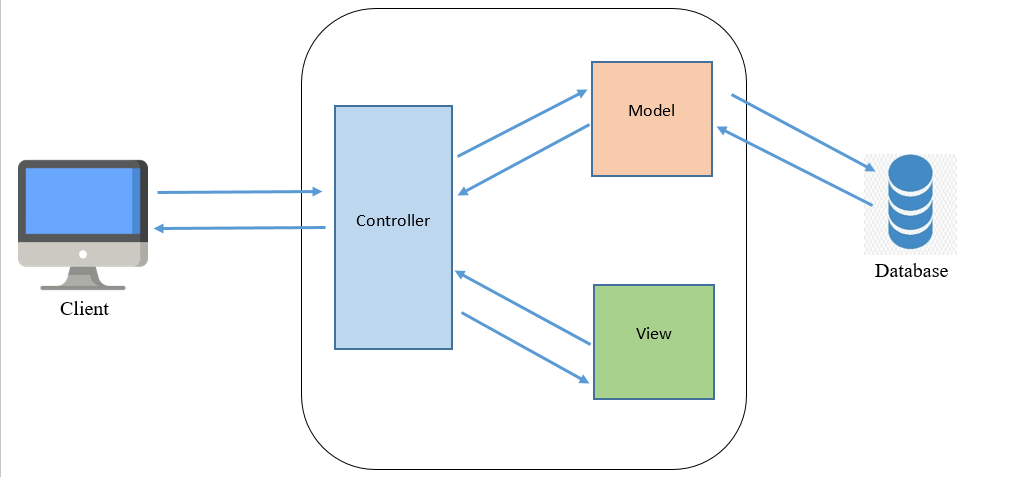
\includegraphics[scale=0.41]{images/mvc.png}
    \caption{Αρχιτεκτονική \engl{MVC}}
    \label{fig:mvc}
\end{figure}

\begin{itemize}
    \item \textbf{\engl{Model}}: Οι συγκεκριμένες κλάσεις χρησιμοποιούνται για την αλληλεπίδραση με τα δεδομένα, δηλαδή την εισαγωγή, την ανάκτηση και την ενημέρωση των βάσεων δεδομένων της εφαρμογής 
    \item \textbf{\engl{View}}: Υλοποιούν με γραφικό τρόπο την διεπαφή της εφαρμογής μέσω της οποίας αλληλεπιδρούν οι χρήστες.
    \item \textbf{\engl{Controller}}: Ακούνε τα αιτήματα των χρηστών και εκτελούν τις κατάλληλες ενέργειες. Οι κλάσεις αυτές αλληλεπιδρούν με τις \engl{Model} και επιλέγουν το κατάλληλο \engl{View} για να εμφανίσουν στον χρήστη ανάλογα με τις ενέργειες που απαιτεί.
\end{itemize}

Βλέπουμε επομένως ότι το \engl{MVC} είναι ένα πρότυπο 3 επιπέδων το οποίο ορίζει εκτός από τα επίπεδα και τις σχέσεις μεταξύ αυτών (Σχήμα \ref{fig:mvc}). Πιο συγκεκριμένα, το επίπεδο του \engl{Controller} αλληλεπιδρά με τον χρήστη λαμβάνοντας δεδομένα τα οποία τα αποστέλλει στο \engl{Model} επίπεδο αφού πρώτα τα επικυρώσει. Επίσης, ανάλογα με το αίτημα του χρήστη θα ζητήσει τα κατάλληλα δεδομένα από το \engl{Model} προκειμένου να τα αποστείλει στο επίπεδο \engl{View} για να δημιουργηθεί η κατάλληλη απεικόνιση για τον χρήστη.

Τέλος, το συγκεκριμένο πρότυπο προσφέρει αρκετά πλεονεκτήματα όπως:

\begin{itemize}
    \item Μας βοηθάει να ελέγξουμε την πολυπλοκότητα της εφαρμογής χωρίζοντας την σε 3 επίπεδα.
    \item Επιτρέπει ευκολότερες δοκιμές (\engl{testing}) της εφαρμογής.
    \item Διαφορετικοί προγραμματιστές μπορούν να δουλεύουν ταυτόχρονα στα διαφορετικά επίπεδα κάτι που μειώνει τον χρόνο ανάπτυξης της εφαρμογής.
    
\end{itemize}

\section{Απαιτήσεις Συστήματος}
Οι απαιτήσεις συστήματος εκφράζουν τις ανάγκες και τους περιορισμούς που τίθενται σε ένα σύστημα το οποίο προσπαθεί να λύσει ένα πραγματικό πρόβλημα \cite{swebok}.

Οι απαιτήσεις από το σύστημα χωρίζονται σε δύο κατηγορίες, τις λειτουργικές (\textbf{ΛΑ}) και τις μη λειτουργικές (\textbf{ΜΛΑ}) απαιτήσεις. Οι λειτουργικές απαιτήσεις αντανακλούν τη δυνατότητα εκτέλεσης ενεργειών που παρέχει το σύστημα στον χρήστη, ενώ οι μη λειτουργικές απαιτήσεις είναι αυτές που χαρακτηρίζουν το σύστημα και προσδιορίζουν ποιοτικά χαρακτηριστικά στις λειτουργίες του. Μπορεί, επίσης, να τεθούν περιορισμοί και στόχοι ως προς τη συμπεριφορά του συστήματος, όπως και απαιτήσεις ως προς την εξελιξιμότητά του.

\subsection{Λειτουργικές Απαιτήσεις}
\subsubsection{\underline{ΛΑ-1}}
Ο χρήστης πρέπει να μπορεί να δίνει φωνητικές εντολές.

\noindent\textbf{Περιγραφή:} Ο χρήστης πρέπει να μπορεί να δίνει φωνητικές εντολής μέσω της φωνής του τις οποίες ο καθρέφτης θα εκτελεί.

\noindent\textbf{\engl{User Priority} (5/5):} Η δυνατότητα φωνητικών εντολών είναι πάρα πολύ σημαντική για τον χρήστη αφού θα είναι ο κύριος τρόπος επικοινωνίας και αλληλεπίδρασής του με τον καθρέφτη.

\noindent\textbf{\engl{Technical Priority} (5/5):} Η δυνατότητα φωνητικών εντολών είναι υψίστης σημασίας για το σύστημα, καθώς πρέπει να είναι σε θέση να αναγνωρίζει τις προθέσεις του χρήστη και να εκτελεί τις κατάλληλες ενέργειες.

\subsubsection{\underline{ΛΑ-2}}
Ο χρήστης πρέπει να μπορεί να ανοίγει διαφορετικές εφαρμογές.

\noindent\textbf{Περιγραφή:} Ο χρήστης πρέπει να μπορεί να χρησιμοποιεί τις διαφορετικές εφαρμογές που είναι εγκατεστημένες στον καθρέφτη.

\noindent\textbf{\engl{User Priority} (5/5):} Η δυνατότητα χρήστης διαφορετικών εφαρμογών είναι πολύ σημαντική για τον χρήστη, καθώς με αυτόν τον τρόπο μπορεί να εκτελέσει τις διαφορετικές λειτουργίες που του παρέχει ο καθρέφτης

\noindent\textbf{\engl{Technical Priority} (5/5):} Η δυνατότητα χρήσης διαφορετικών εφαρμογών είναι πολύ σημαντική για το σύστημα, αφού θα πρέπει να είναι σε θέση να εκτελεί τις διαφορετικές εφαρμογές που είναι εγκατεστημένες στον καθρέφτη.

\subsubsection{\underline{ΛΑ-3}}
Ο χρήστης πρέπει να μπορεί να εγκαθιστά διαφορετικές εφαρμογές.

\noindent\textbf{Περιγραφή:} Ο χρήστης πρέπει να μπορεί να εγκαθιστά στον καθρέφτη εφαρμογές που αναπτύσσει αυτός ή κάποιος τρίτος.

\noindent\textbf{\engl{User Priority} (4/5):} Η δυνατότητα εγκατάστασης διαφορετικών εφαρμογών είναι αρκετά σημαντική για τον χρήστη, καθώς με αυτόν τον τρόπο θα μπορεί να επεκτείνει τις δυνατότητες του καθρέφτη.

\noindent\textbf{\engl{Technical Priority} (5/5):} Η δυνατότητα εγκατάστασης διαφορετικών εφαρμογών είναι πολύ σημαντική για το σύστημα, αφού θα πρέπει να δέχεται εύκολα εξωτερικές εφαρμογές και να τις εκτελεί χωρίς προβλήματα. 

\subsubsection{\underline{ΛΑ-4}}
Ο χρήστης πρέπει να μπορεί να ενεργοποιεί και να απενεργοποιεί τον καθρέφτη με φωνητικές εντολές.

\noindent\textbf{Περιγραφή:} Ο χρήστης πρέπει να μπορεί να ενεργοποιεί και να απενεργοποιεί τον καθρέφτη δίνοντάς του κατάλληλες εντολές ανοίγματος/κλεισίματος.

\noindent\textbf{\engl{User Priority} (5/5):} Η δυνατότητα ενεργοποίησης/απενεργοποίησης του καθρέφτη με εντολές είναι πολύ σημαντική για τον χρήστη, καθώς θα μπορεί να ελέγξει πότε ο καθρέφτης να είναι σε λειτουργία

\noindent\textbf{\engl{Technical Priority} (5/5):} Η δυνατότητα ενεργοποίησης/απενεργοποίησης του καθρέφτη με εντολές είναι πολύ σημαντική για το σύστημα, καθώς θα μπορεί να ελεγχθεί η κατάσταση λειτουργίας του.

\subsubsection{\underline{ΛΑ-5}}
Ο χρήστης πρέπει να μπορεί να αλλάζει τις ρυθμίσεις του καθρέφτη.

\noindent\textbf{Περιγραφή:} Ο χρήστης πρέπει να μπορεί να αλλάζει τις ρυθμίσεις του καθρέφτη είτε μέσω εντολών είτε μέσω κειμένου.

\noindent\textbf{\engl{User Priority} (5/5):} Η δυνατότητα αλλαγής των ρυθμίσεων είναι πολύ σημαντική για τον χρήστη, καθώς θα μπορεί να εξατομικεύσει τις λειτουργίες του καθρέφτη ανάλογα με τα θέλω του.

\noindent\textbf{\engl{Technical Priority} (5/5):} Η δυνατότητα αλλαγής των ρυθμίσεων είναι πολύ σημαντική για το σύστημα, καθώς θα είναι εφικτή η ορθή και εξατομικευμένη λειτουργία των εφαρμογών του καθρέφτη.

\subsubsection{\underline{ΛΑ-6}}
Ο χρήστης πρέπει να μπορεί να δει την ημερομηνία και ώρα

\noindent\textbf{Περιγραφή:} Ο χρήστης πρέπει να μπορεί να δει την τωρινή ημερομηνία και την ώρα στην αρχική οθόνη του καθρέφτη

\noindent\textbf{\engl{User Priority} (5/5):} Η δυνατότητα ενημέρωσης για την ημερομηνία και ώρα είναι πολύ σημαντική για τον χρήστη προκειμένου να μπορεί να οργανώσει καλύτερα το πρόγραμμά του.

\noindent\textbf{\engl{Technical Priority} (5/5):} Η δυνατότητα ενημέρωσης για την ημερομηνία και ώρα είναι πολύ σημαντική για το σύστημα αφού με βάση αυτά μπορεί να επηρεαστεί η λειτουργία του.

\subsubsection{\underline{ΛΑ-7}}
Ο χρήστης πρέπει να μπορεί να δει τον καιρό σε ζωντανό χρόνο.

\noindent\textbf{Περιγραφή:} Ο χρήστης πρέπει να μπορεί να δει τον καιρό σε ζωντανό χρόνο στην αρχική οθόνη του καθρέφτη.

\noindent\textbf{\engl{User Priority} (5/5):} Η δυνατότητα ζωντανής ενημέρωσης του καιρού είναι πολύ σημαντική για τον χρήστη, καθώς μπορεί να οργανώσει καλύτερα το πρόγραμμά του.

\noindent\textbf{\engl{Technical Priority} (4/5):} Η δυνατότητα ζωντανής ενημέρωσης του καιρού είναι αρκετά σημαντική για το σύστημα αφού μπορεί να χρησιμοποιήσει τις πληροφορίες για βελτίωση της λειτουργίας του

\subsubsection{\underline{ΛΑ-8}}
Ο χρήστης πρέπει να μπορεί να κάνει ερωτήσεις σχετικά με τον καιρό.

\noindent\textbf{Περιγραφή:} Ο χρήστης πρέπει να μπορεί να κάνει ερωτήσεις και να ενημερώνεται σχετικά με τον καιρό.

\noindent\textbf{\engl{User Priority} (4/5):} Η δυνατότητα ερωτήσεων σχετικά με τον καιρό είναι αρκετά σημαντική για τον χρήστη αφού μπορεί να ενημερωθεί και να οργανώσει καλύτερα το πρόγραμμά του.

\noindent\textbf{\engl{Technical Priority} (2/5):} Η δυνατότητα ερωτήσεων σχετικά με τον καιρό δεν είναι πολύ σημαντική για την εύρυθμη λειτουργία του συστήματος αφού μπορεί να λειτουργήσει ομαλά και χωρίς αυτήν.


\subsubsection{\underline{ΛΑ-9}}
Ο χρήστης πρέπει να μπορεί να

\noindent\textbf{Περιγραφή:}

\noindent\textbf{\engl{User Priority} (5/5):}

\noindent\textbf{\engl{Technical Priority} (4/5):}

\subsubsection{\underline{ΛΑ-10}}
Ο χρήστης πρέπει να μπορεί να

\noindent\textbf{Περιγραφή:}

\noindent\textbf{\engl{User Priority} (5/5):}

\noindent\textbf{\engl{Technical Priority} (4/5):}

\subsubsection{\underline{ΛΑ-11}}
Ο χρήστης πρέπει να μπορεί να

\noindent\textbf{Περιγραφή:}

\noindent\textbf{\engl{User Priority} (5/5):}

\noindent\textbf{\engl{Technical Priority} (4/5):}

\subsubsection{\underline{ΛΑ-12}}
Ο χρήστης πρέπει να μπορεί να

\noindent\textbf{Περιγραφή:}

\noindent\textbf{\engl{User Priority} (5/5):}

\noindent\textbf{\engl{Technical Priority} (4/5):}


\noindent\subsection{Μη Λειτουργικές Απαιτήσεις}

\subsubsection{\underline{ΜΛΑ-1}}
Το σύστημα πρέπει να αποκρίνεται στις εντολές του χρήστη σε λιγότερο από 500\engl{ms}.

\noindent\textbf{Περιγραφή:} Το σύστημα πρέπει να αναγνωρίζει τις προθέσεις του χρήστη και να ανταποκρίνεται κατάλληλα σε λιγότερο από 500\engl{ms}.

\noindent\textbf{\engl{User Priority} (5/5):} Η απαίτηση αυτή είναι πολύ σημαντική για τον χρήστη, καθώς θέλει ο καθρέφτης να του προσφέρει μια διαδραστική εμπειρία πραγματικού χρόνου.

\noindent\textbf{\engl{Technical Priority} (5/5):} Η απαίτηση αυτή είναι πολύ σημαντική για το σύστημα, καθώς θα καθορίσει τα τεχνικά χαρακτηριστικά και τη δομή του, προκειμένου να καλύπτεται η απαιτούμενη ταχύτητα απόκρισης (500\engl{ms}).

\subsubsection{\underline{ΜΛΑ-2}}
Το σύστημα πρέπει να ανταποκρίνεται ορθά όταν η εντολή του χρήστη δεν αναγνωρίζεται

\noindent\textbf{Περιγραφή:} Το σύστημα πρέπει να χειρίζεται εντολές του χρήστη που δεν αναγνωρίζονται και να μην καταρρέει.

\noindent\textbf{\engl{User Priority} (5/5):} Η απαίτηση αυτή είναι πολύ σημαντική για τον χρήστη, καθώς θέλει ο καθρέφτης να λειτουργεί χωρίς σφάλματα.

\noindent\textbf{\engl{Technical Priority} (5/5):} Η απαίτηση αυτή είναι πολύ σημαντική για το σύστημα, καθώς ο χειρισμός των "κακών" εισόδων θα βοηθήσει τον καθρέφτη να λειτουργεί ορθά χωρίς σφάλματα.

\subsubsection{\underline{ΜΛΑ-3}}
Το σύστημα πρέπει να επιτρέπει την προσάρτηση εφαρμογών.

\noindent\textbf{Περιγραφή:} Το σύστημα πρέπει να επιτρέπει την προσάρτηση εφαρμογών και την εύκολη ενσωμάτωσή τους στην ροή του προγράμματος.

\noindent\textbf{\engl{User Priority} (5/5):} Η απαίτηση αυτή είναι πολύ σημαντική για τον χρήστη, καθώς η ενσωμάτωση εξωτερικών εφαρμογών θα επεκτείνει τις δυνατότητες που θα του δίνει ο καθρέφτης.

\noindent\textbf{\engl{Technical Priority} (5/5):} Η απαίτηση αυτή είναι πολύ σημαντική για το σύστημα, καθώς θα πρέπει να σχεδιαστεί με τέτοιο τρόπο ώστε να είναι εύκολη η επεκτασιμότητα των εφαρμογών του καθρέφτη.

\subsubsection{\underline{ΜΛΑ-4}}
Το σύστημα πρέπει να επιτρέπει την ταυτόχρονη εμφάνιση εφαρμογών και του ειδώλου του χρήστη.

\noindent\textbf{Περιγραφή:} Το σύστημα πρέπει να έχει ανακλαστική οθόνη στην οποία ο χρήστης να μπορεί να δει τόσο τις εφαρμογές του καθρέφτη όσο και το είδωλό του.

\noindent\textbf{\engl{User Priority} (5/5):} Η απαίτηση αυτή είναι πολύ σημαντική για τον χρήστη, καθώς θέλει να μπορεί να αλληλεπιδρά με τον καθρέφτη καθώς βλέπει το είδωλό του.

\noindent\textbf{\engl{Technical Priority} (5/5):} Η απαίτηση αυτήν είναι πολύ σημαντική για το σύστημα, καθώς θα καθορίσει το είδος της οθόνης που θα χρησιμοποιηθεί και την τοποθέτηση των εφαρμογών πάνω σε αυτήν.

\subsubsection{\underline{ΜΛΑ-5}}
Το σύστημα πρέπει να υποστηρίζει σύνδεση με το \engl{Wit.ai}.

\noindent\textbf{Περιγραφή:} Το σύστημα πρέπει να υποστηρίζει σύνδεση με το \engl{Wit.ai} προκειμένου να επιτρέπεται η αναγνώριση πρόθεσης των εντολών του χρήστη.

\noindent\textbf{\engl{User Priority} (5/5):} Η απαίτηση αυτή είναι πολύ σημαντική για τον χρήστη, καθώς ο καθρέφτης πρέπει να αναγνωρίζει τις προθέσεις του και να εκτελεί τις κατάλληλες ενέργειες.

\noindent\textbf{\engl{Technical Priority} (5/5):} Η απαίτηση αυτή είναι πολύ σημαντική για το σύστημα, καθώς πρέπει να μπορεί να αναγνωρίζει τις προθέσεις του χρήστη για να εκτέλεση των επιθυμητών ενεργειών.

\subsubsection{\underline{ΜΛΑ-6}}
Το σύστημα πρέπει να λειτουργεί μόνο όταν ανιχνεύει πρόσωπο ανθρώπου.

\noindent\textbf{Περιγραφή:} Το σύστημα πρέπει να ανιχνεύει την ύπαρξη ανθρώπου μπροστά στον καθρέφτη και να σταματά τη λειτουργία του όταν δεν βρίσκει τίποτα.

\noindent\textbf{\engl{User Priority} (4/5):} Η απαίτηση αυτή είναι σημαντική για τον χρήστη, καθώς δεν επιθυμεί ο καθρέφτης να ανιχνεύει τα λόγια του σε ανύποπτο χρόνο και να πιάνει εντολές χωρίς πρόθεση.

\noindent\textbf{\engl{Technical Priority} (5/5):} Η απαίτηση αυτήν είναι πολύ σημαντική για το σύστημα, καθώς θα πρέπει να ελέγχει συνεχώς την ύπαρξη χρήστη μπροστά στον καθρέφτη και να σταματά τη λειτουργία του. Η απαίτηση αυτή θα βοηθήσει και στην εξοικονόμηση πόρων του συστήματος.

\subsubsection{\underline{ΜΛΑ-7}}
Το σύστημα πρέπει να συνδέεται στο διαδίκτυο με ικανοποιητικό εύρος σύνδεσης.

\noindent\textbf{Περιγραφή:} Το σύστημα πρέπει να υποστηρίζει σύνδεση στο διαδίκτυο προκειμένου να μπορεί να αλληλεπιδρά με τα διαφορετικά \engl{APIs} και να λειτουργεί ορθά. Επομένως πρέπει να υπάρχει η απαραίτητη υποστήριξη σύνδεσης στο διαδίκτυο από το υλικό του συστήματος.

\noindent\textbf{\engl{User Priority} (5/5):} Η απαίτηση αυτή είναι πολύ σημαντική για τον χρήστη, καθώς χωρίς σύνδεση διαδικτύου ο καθρέφτης δεν θα είναι σε θέση να εκτελέσει τις εφαρμογές του και να αναγνωρίσει τις εντολές του χρήστη.

\noindent\textbf{\engl{Technical Priority} (5/5):} Η απαίτηση αυτή είναι πολύ σημαντική για το σύστημα, καθώς χρειάζεται σύνδεση στο διαδίκτυο για να λειτουργήσει ο καθρέφτης τις εφαρμογές του. 

\subsubsection{\underline{ΜΛΑ-8}}
Το σύστημα πρέπει να 

\noindent\textbf{Περιγραφή:}

\noindent\textbf{\engl{User Priority} (5/5):}

\noindent\textbf{\engl{Technical Priority} (4/5):}

\section{Μοντελοποίηση Κλάσεων}
Η οργάνωση του κώδικα έγινε με την μορφή κλάσεων στη γλώσσα \engl{Python} ενώ όπως έχει αναφερθεί παραπάνω για την γραφική διεπαφή χρησιμοποιήθηκε η βιβλιοθήκη \engl{Kivy}. Στο παρόν κεφάλαιο θα παρουσιαστούν όλες οι κλάσεις που υλοποιήθηκαν για το λογισμικό του καθρέφτη μαζί με τις μεταβλητές και μεθόδους που ανήκουν σε κάθε κλάση, ενώ θα γίνει και μια περιγραφή του κάθε μέλους. Με τέτοιου είδους διαγράμματα είναι εφικτό να μοντελοποιηθεί το λογισμικό σε ανώτερο επίπεδο και χωρίς να χρειαστεί να κοιτάξουμε άμεσα τον κώδικα \cite{ClassDiagrams}. Η περιγραφή των κλάσεων θα γίνει στην γλώσσα \engl{UML\footnote{\href{https://en.wikipedia.org/wiki/Unified\_Modeling\_Language}{https://en.wikipedia.org/wiki/Unified\_Modeling\_Language}}} κατά την οποία, όπως φαίνεται στο Σχήμα \ref{fig:class_diagram_example}, μια κλάση αναπαριστάται από 3 μέρη, το όνομά της, τα χαρακτηριστικά (μεταβλητές) της και τέλος οι μέθοδοί της.

\begin{figure}[h]
    \centering
    
\includegraphics[scale=0.1]{images/uml_diagrams/class_diagram_example.png}
    \caption{Παράδειγμα αναπαράστασης κλάσης στη \engl{UML}}
    \label{fig:class_diagram_example}
\end{figure}

\subsection{\texorpdfstring{\engl{SmartMirrorApp}}{SmartMirrorApp}}

\begin{figure}[h]
    \centering
    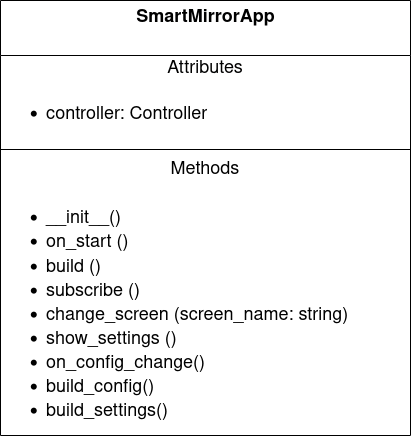
\includegraphics[scale=0.7]{images/uml_diagrams/SmartMirrorApp.png}
    \caption{\engl{UML} της κλάσης \engl{SmartMirrorApp}}
    \label{fig:smartmirrorapp}
\end{figure}
\noindent\textbf{Περιγραφή Κλάσης}

Η κλάση αυτή κληρονομεί από την κλάση \engl{\href{https://kivy.org/doc/stable/api-kivy.app.html\#kivy.app.App}{\texttt{kivy.app.App}}} η οποία είναι η βασική κλάση για την δημιουργία μιας \engl{Kivy} εφαρμογής. Μέσως αυτής της κλάσης ελέγχουμε την γραφική εφαρμογή και όταν όλα είναι έτοιμα ξεκινάμε τον κύκλο ζωής της εφαρμογής καλώντας την μέθοδο \engl{\texttt{SmartMirrorApp().run()}}.

\noindent\textbf{Χαρακτηριστικά Κλάσης}
\begin{itemize}
    \item \engl{\texttt{controller}}: Αντικείμενο τύπου \engl{Controller} για την ενεργοποίηση του \engl{thread} ελέγχου.
\end{itemize}

\noindent\textbf{Μέθοδοι Κλάσης}
\begin{itemize}
    \item \engl{\texttt{\_\_init\_\_()}}: Συνάρτηση δόμησης της κλάσης η οποία καλή την συνάρτηση δόμησης της κλάσης \engl{\texttt{kivy.app.App}} μέσω του \engl{\texttt{super()}} και αρχικοποιεί τη μεταβλητή \engl{\texttt{controller}} να είναι \engl{\texttt{None}}.
    
    \item \engl{\texttt{on\_start()}}: Ειδική μέθοδος της κλάσης \engl{\texttt{kivy.app.App}} που εκτελείται λίγο πριν την εκκίνηση της εφαρμογής (αμέσως μετά την συνάρτηση \engl{\texttt{build()}}. Δημιουργεί το αντικείμενο \engl{\texttt{Controller}} και ξεκινάει το \engl{thread} ελέγχου.
    
    \item \engl{\texttt{build()}}: Ειδική μέθοδος της κλάσης \engl{\texttt{kivy.app.App}} η οποία αρχικοποιεί την εφαρμογή και εκτελείται μόνο μία φορά. Φορτώνει όλες τις εγκατεστημένες εφαρμογές και επιστρέφει το βασικό \engl{Widget} (ένα στιγμιότυπο της κλάσης \engl{MainPage} η οποία θα εξηγηθεί παρακάτω).
    
    \item \engl{\texttt{subscribe()}}: Μέθοδος η οποία επιστρέφει ένα \engl{Python dictionary} όπου γίνεται μια αντιστοίχηση ενός \engl{intent} σε μια συνάρτηση. Η μέθοδος αυτή χρησιμοποιείται προκειμένου να μπορεί να εκτελεστεί η σωστή συνάρτηση όταν γίνει αναγνώριση της πρόθεσης της εντολής του χρήστη από το \engl{Wit.ai}. 
    
    \item \engl{\texttt{change\_screen(screen\_name: string)}}: Συνάρτηση που χρησιμοποείται για να γίνει αλλαγή \engl{Screen} δηλαδή να φορτώσει μια άλλη εφαρμογή με όνομα \engl{\texttt{screen\_name}}.
    
    \item \engl{\texttt{show\_settings()}}: Μέθοδος η οποία καλεί την συνάρτηση \engl{\texttt{open\_settings()}} της κλάσης \engl{\texttt{kivy.app.App}} για να ανοίξει το μενού ρυθμίσεων της εφαρμογής.
    
    \item \engl{\texttt{on\_config\_change()}}: Ειδική μέθοδος της κλάσης \engl{\texttt{kivy.app.App}} η οποία εκτελείται όταν γίνει κάποια αλλαγή ρύθμισης. Για κάθε ένα από τα εγκατεστημένα \engl{Widgets} ανανεώνει τις ρυθμίσεις τους.
    
    \item \engl{\texttt{build\_config()}}: Ειδική μέθοδος της κλάσης \engl{\texttt{kivy.app.App}} η οποία
    εκτελείται πριν την αρχικοποίηση της εφαρμογής και δημιουργεί \engl{default} ρυθμίσεις για κάθε ένα από τα εγκατεστημένα \engl{Widgets}.
    
    \item \engl{\texttt{build\_settings()}}: Ειδική μέθοδος της κλάσης \engl{\texttt{kivy.app.App}} η οποία εκτελείται όταν θέλουμε να δείξουμε τις ρυθμίσεις της εφαρμογής. Διαβάζει από κάθε εγκατεστημένο \engl{Widget} τις ρυθμίσεις τους (οι οποίες βρίσκονται σε ένα αρχείο \engl{"settings.json"} και τις προσθέτει στο μενού ρυθμίσεων.
    
\end{itemize}

\newpage
\subsection{\texorpdfstring{\engl{MainPage}}{MainPage}}

\begin{figure}[h]
    \centering
    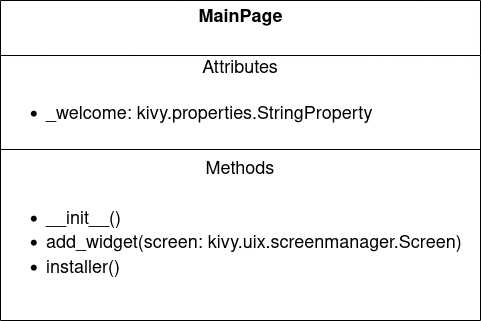
\includegraphics[scale=0.7]{images/uml_diagrams/MainPage.png}
    \caption{\engl{UML} της κλάσης \engl{MainPage}}
    \label{fig:mainpage}
\end{figure}

\noindent\textbf{Περιγραφή Κλάσης}

Η κλάση αυτή κληρονομεί από την κλάση \engl{\href{https://kivy.org/doc/stable/api-kivy.uix.screenmanager.html\#kivy.uix.screenmanager.ScreenManager}{ScreenManager}} που περιέχεται στο πακέτο \engl{\texttt{kivy.uix.screenmanager}}. Η κλάση αυτή είναι το πρωτεύον \engl{Widget} που επιστρέφει η εφαρμογή και κάτω από αυτήν μπαίνουν όλες οι εφαρμογές που εγκαθιστά ο χρήστης (σαν καινούργια \engl{Screens}).

\noindent\textbf{Χαρακτηριστικά Κλάσης}
\begin{itemize}
    \item \engl{\texttt{\_welcome}}: Μεταβλητή που χρησιμοποιείται για να αποθηκεύσει ένα μήνυμα που καλωσορίζει τον χρήστη.
\end{itemize}

\noindent\textbf{Μέθοδοι Κλάσης}
\begin{itemize}
    \item \engl{\texttt{\_\_init\_\_()}}: Η συνάρτηση δόμησης της κλάσης η οποία καλή την συνάρτηση δόμησης της κλάσης \engl{\texttt{kivy.uix.screenmanager.ScreenManager}} μέσω του \engl{\texttt{super()}} και αρχικοποιεί τη μεταβλητή \engl{\texttt{\_welcome}} να πάρει μία τυχαία επιλογή από μια λίστα μηνυμάτων. Τέλος καλεί την εσωτερική συνάρτηση \engl{\texttt{installer}} προκειμένου να εγκαταστήσει όλες τις εφαρμογές που βρίσκονται στον φάκελο \engl{\texttt{/widgets}} σαν ξεχωριστά \engl{Screens}.
    
    \item \engl{\texttt{add\_widget(screen: kivy.uix.screenmanager.Screen)}}: Ειδική συνάρτηση της κλάσης \engl{\texttt{kivy.uix.screenmanager.ScreenManager}} η οποία προσθέτει ένα καινούργιο \engl{Widget} στα παιδιά του τρέχοντος \engl{Widget}. Στην υπερφορτωμένη της έκδοση, επιτρέπεται η πρόσθεση μόνο \engl{Widget} τύπου \engl{\texttt{kivy.uix.screenmanager.Screen}} για περισσότερη ασφάλεια.
    
    \item \engl{\texttt{installer()}}: Συνάρτηση η οποία για κάθε ένα από τα παιδιά της \engl{\texttt{MainPage}} καλεί την συνάρτηση \engl{\texttt{install}} την οποία πρέπει να ορίσουν οι εξωτερικές εφαρμογές προκειμένου να μπορούν να εγκατασταθούν από τον καθρέφτη.
\end{itemize}

\subsection{\texorpdfstring{\engl{Controller}}{Controller}}
\begin{figure}[h]
    \centering
    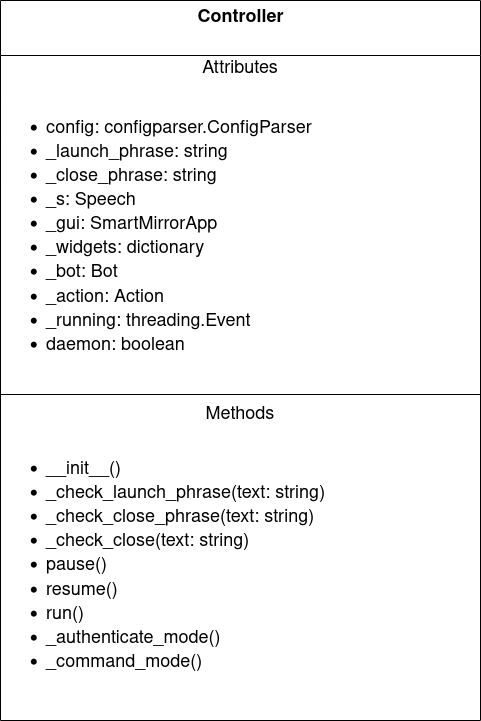
\includegraphics[scale=0.7]{images/uml_diagrams/Controller.png}
    \caption{\engl{UML} της κλάσης \engl{Controller}}
    \label{fig:controller}
\end{figure}
\noindent\textbf{Περιγραφή Κλάσης}

Η κλάση αυτή κληρονομεί από την κλάση \engl{\href{https://docs.python.org/3/library/threading.html\#threading.Thread}{threading.Thread}}. O \engl{controller} είναι ένα ανεξάρτητο \engl{thread} από το \engl{main thread} στο οποίο τρέχει η γραφική εφαρμογή και είναι υπεύθυνος για τον έλεγχο των λειτουργιών του συστήματος. Μέσα από αυτήν την κλάση ελέγχεται η ροή του προγράμματος, επιλέγονται οι ενέργειες που θα εκτελέσει ο καθρέφτης και ανανεώνεται το γραφικό περιβάλλον με βάση τις εντολές του χρήστη.

\noindent\textbf{Χαρακτηριστικά Κλάσης}
\begin{itemize}
    \item \engl{\texttt{config}}: Αντικείμενο τύπου \engl{\texttt{configparser.ConfigParser}} για την ανάγνωση ρυθμίσεων.
    \item \engl{\texttt{\_launch\_phrase}}: Μεταβλητή για την αποθήκευση της φράσης ενεργοποίησης του καθρέφτη.
    \item \engl{\texttt{\_close\_phrase}}: Μεταβλητή για την αποθήκευση της φράσης απενεργοποίησησς του καθρέφτη.
    \item \engl{\texttt{\_s}}: Αντικείμενο τύπου \engl{\texttt{Speech}} το οποίο χρησιμοποιείται για την αναγνώριση της φωνής του χρήστη.
    \item \engl{\texttt{\_gui}}: Αντικείμενο τύπου \engl{\texttt{SmartMirrorApp}} το οποίο χρησιμοποιείται για να γίνεται αλληλεπίδραση μεταξύ του \engl{Controller} και του γραφικού περιβάλλοντος.
    \item \engl{\texttt{\_widgets}}: \engl{Dictionary} το οποίο αποθηκεύει όλα τα \engl{Widgets} του γραφικού περιβάλοντος με τα \engl{ids} τους ως κλειδιά.
    \item \engl{\texttt{\_bot}}: Αντικείμενο τύπου \engl{\texttt{Bot}} το οποίο χρησιμοποιείται για την αλληλεπίδραση με το \engl{Wit.ai}.
    \item \engl{\texttt{\_action}}: Αντικείμενο τύπου \engl{\texttt{Action}} το οποίο χρησιμοποιείται ως βοηθημα για την εκτέλεση της εντολής του χρήστη.
    \item \engl{\texttt{\_running}}: Μεταβλητή τύπου \engl{\texttt{threading.Event}} η οποία χρησιμοποιείται για τον έλεγχο του \engl{Thread} του \engl{Controller}.
    \item \engl{\texttt{daemon}}: Μεταβλητή που καθορίζει αν το \engl{Thread} θα εκτελεστεί στο προσκήνιο ή στο παρασκήνιο.
\end{itemize}
\noindent\textbf{Μέθοδοι Κλάσης}
\begin{itemize}
    \item \engl{\texttt{\_\_init\_\_()}}: Η συνάρτηση δόμησης της κλάσης διαβάζει από τις ρυθμίσεις τις φράσεις ενεργοποίησης/απενεργοποίησης, αρχικοποιεί τα αντικείμενα των βοηθητικών κλάσεων που θα χρησιμοποιηθούν για τον έλεγχο του καθρέφτη και τέλος ξεκινάει ένα \engl{Thread} στο παρασκήνιο στο οποίο θα γίνεται ο λογικός έλεγχος της ροής του προγράμματος.
    \item \engl{\texttt{\_check\_launch\_phrase(text: String)}}: Βοηθητική συνάρτηση όπου επιστρέφει \engl{True} αν η μεταβλητή \engl{\texttt{text}} ταυτίζεται με την φράση έναρξης και \engl{False} σε αντίθετη περίπτωση.
    \item \engl{\texttt{\_check\_close\_phrase(text: String)}}: Βοηθητική συνάρτηση όπου επιστρέφει \engl{True} αν η μεταβλητή \engl{\texttt{text}} ταυτίζεται με την φράση απενεργοποίησης και \engl{False} σε αντίθετη περίπτωση.
    \item \engl{\texttt{\_check\_close(text: String)}}: Βοηθητική συνάρτηση που ελέγχει εαν η μεταβλητή \engl{\texttt{text}} είναι ίση με \engl{\texttt{\"quit\"}} ή \engl{\texttt{\"exit\"}} προκειμένου να διακόψει τη λειτουργία του καθρέφτη.
    \item \engl{\texttt{pause()}}: Βοηθητική συνάρτηση η οποία σταματάει το \engl{Thread} του \engl{Controller}.
    \item \engl{\texttt{resume()}}: Βοηθητική συνάρτηση η οποία ενεργοποιεί το \engl{Thread} του \engl{Controller}.
    \item \engl{\texttt{run()}}: H συνάρτηση αυτή ενεργοποιεί το \engl{Thread} του \engl{Controller} και καλεί τις συναρτήσεις \engl{\texttt{\_authenticate\_mode()}} και \engl{\texttt{\_command\_mode()}} η οποίες ελέγχουν την κατάσταση του καθρέφτη.
    \item \engl{\texttt{\_authenticate\_mode()}}: Στη συγκεκριμένη κατάσταση ο καθρέφτης είναι αδρανής και περιμένει να ακούσει την φράση ενεργοποίησης προκειμένου να δώσει πρόσβαση στον χρήστη και να ακολουθεί τις εντολές του. Με αυτόν τον τρόπο ο καθρέφτης θα ακούει τις εντολές του χρήστη μόνο όταν αυτός το θέλει.
    \item \engl{\texttt{\_command\_mode()}}: Στη συγκεκριμένη κατάσταση γίνεται ο έλεγχος της ροής του καθρέφτη όπου γίνεται επαναληπτικά η ακοή της εντολής του χρήστη, η αλληλεπίδραση με το \engl{Wit.ai} για την αναγνώριση της πρόθεσης του χρήστη και η εκτέλεση της εντολής αν αυτή είναι αποδεκτή. Η επανάληψη συνεχίζεται έως ότου ο χρήστης πει την φράση απενεργοποίησης ή μία εκ των εντολών \engl{"quit"} και \engl{"exit"} οι οποίες απενεργοποιούν τον καθρέφτη.
\end{itemize}
\newpage
\subsection{\texorpdfstring{\engl{Speech}}{Speech}}
\begin{figure}[h]
    \centering
    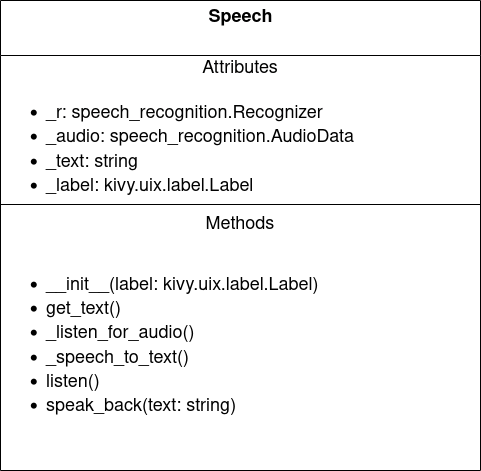
\includegraphics[scale=0.7]{images/uml_diagrams/Speech.png}
    \caption{\engl{UML} της κλάσης \engl{Speech}}
    \label{fig:speech}
\end{figure}
\noindent\textbf{Περιγραφή Κλάσης}

Η κλάση αυτή υλοποιεί όλες τις μεθόδους και την διεπαφή για την ανάγνωση και ομιλία ήχου. Μέσω αυτής της κλάσης ο καθρέφτης μπορεί να ακούει τον χρήστη από το μικρόφωνο ανά τακτά διαστήματα και να μετατρέπει τις εντολές του σε κείμενο το οποίο θα χρησιμοποιηθεί αργότερα για την αναγνώριση της πρόθεσης. Τέλος, μέσω αυτής της κλάσης ο καθρέφτης δύναται να μιλήσει στον χρήστη, λέγοντάς του αποτελέσματα ενεργειών ή πληροφορίες.

\noindent\textbf{Χαρακτηριστικά Κλάσης}
\begin{itemize}
    \item \engl{\texttt{\_r}}: Αντικείμενο τύπου \engl{\texttt{speech\_recognition.Recognizer}} μέσω του οποίο γίνεται η ανάγνωση της φωνής και η αναγνώρισή της σε κείμενο.
    \item \engl{\texttt{\_audio}}: Αντικείμενο τύπου \engl{\texttt{speech\_recognition.AudioData}} το οποίο αποθηκεύει τα δεδομένα του ήχου τα οποία χρησιμοποιούνται για την αναγνώριση και μετατροπή σε κείμενο.
    \item \engl{\texttt{\_text}}: Μεταβλητή στην οποία αποθηκεύεται σε γραπτή μορφή η εντολή του χρήστη μετά την αναγνώριση.
    \item \engl{\texttt{\_label}}: Αντικείμενο τύπου \engl{\texttt{kivy.uix.label.Label}} το οποίο χρησιμοποιείται προκειμένου να εμφανίζεται στην οθόνη του καθρέφτη πότε το σύστημα ακούει εντολές από τον χρήστη.
\end{itemize}
\noindent\textbf{Μέθοδοι Κλάσης}
\begin{itemize}
    \item \engl{\texttt{\_\_init\_\_(kivy.uix.label.Label)}}: Συνάρτηση δόμησης της κλάσης η οποία αρχικοποιεί τις μεταβλητές που χρησιμποιεί η κλάση και δέχεται ως είσοδο το \engl{Label} στο οποίο θα υποδηλώνεται πότε ο καθρέφτης ακούει για εντολές.
    \item \engl{\texttt{get\_text()}}: Βοηθητική συνάρτηση η οποία επιστρέφει την τιμή της μεταβλητής \engl{\texttt{\_text}}.
    \item \engl{\texttt{\_listen\_for\_audio()}}: Συνάρτηση η οποία ακούει από το μικρόφωνο τις εντολές του χρήστη. Η λειτουργία ανάγνωσης του ήχου από το μικρόφωνο του συστήματος γίνεται με την αρχικοποίηση ενός αντικειμένου τύπου \engl{\texttt{speech\_recognition.Microphone}}. Τα δεδομένα ήχου αποθηκεύονται στο αντικείμενο \engl{\texttt{\_audio}} ενώ γίνεται και εγγραφή στο \engl{Label} του καθρέφτη για την ενημέρωση του χρήστη ότι το σύστημα περιμένει εντολή.
    \item \engl{\texttt{\_speech\_to\_text()}}: Η συνάρτηση αυτή καλεί την μέθοδο \engl{\texttt{recognize\_google()}} του αντικειμένου \engl{\texttt{\_r}} η οποία αλληλεπιδρά με το \engl{API} της \engl{Google} για την μετατροπή των δεδομένων ήχου σε κείμενο. Σε περίπτωση που δεν γίνεται αναγνώριση το κείμενο τίθεται κενό.
    \item \engl{\texttt{listen()}}: Συνάρτηση η οποία καλείται από τον \engl{Controller} και καλεί τις 2 συναρτήσεις για ανάγνωση του ήχου και μετατροπή σε κείμενο.
    \item \engl{\texttt{speak\_back(text: string)}}: Συνάρτηση η οποία καλείται εξωτερικά για την ομιλία του καθρέφτη προς τον χρήστη. Μέσω της βιβλιοθήκης \engl{gTTS} μετατρέπεται το κειμενο εισόδου σε ομιλία, αποθηκεύεται ως ένα προσωρινό αρχείο \engl{.mp3} και αναπαράγεται μέσω της βιβλιοθήκης \engl{pydub}. Τέλος, το προσωρινό αρχείο διαγράφεται.
\end{itemize}
\newpage
\subsection{\texorpdfstring{\engl{Bot}}{Bot}}
\begin{figure}[h]
    \centering
    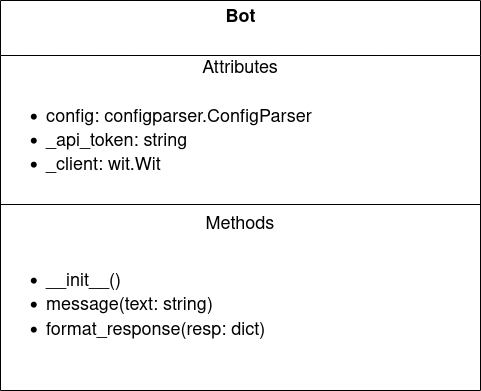
\includegraphics[scale=0.7]{images/uml_diagrams/Bot.png}
    \caption{\engl{UML} της κλάσης \engl{Bot}}
    \label{fig:bot}
\end{figure}
\noindent\textbf{Περιγραφή Κλάσης}

Η κλάση αυτή αποτελεί την διεπαφή για την αλληλεπίδραση με το \engl{Wit.ai} και την εξαγωγή της πρόθεσης της εντολής του χρήστη αλλά και των οντοτήτων οι οποίες θα δοθούν ως ορίσματα κατά την εκτέλεση των εντολών.

\noindent\textbf{Χαρακτηριστικά Κλάσης}
\begin{itemize}
    \item \engl{\texttt{config}}: Αντικείμενο τύπου \engl{\texttt{configparser.ConfigParser}} για την ανάγνωση ρυθμίσεων.
    \item \engl{\texttt{\_api\_token}}: Μεταβλητή η οποία αποθηκεύει το \engl{api\_key} που χρησιμοποιείται για να αποκτήσει η εφαρμογή πρόσβαση στο \engl{Wit.ai}.
    \item \engl{\texttt{\_client}}: Αντικείμενο τύπου \engl{\texttt{wit.Wit}} μέσω του οποίου θα γίνεται η αλληλεπίδραση με το \engl{Wit.ai}.
\end{itemize}
\noindent\textbf{Μέθοδοι Κλάσης}
\begin{itemize}
    \item \engl{\texttt{\_\_init\_\_()}}: Συνάρτηση δόμησης της κλάσης η οποία διαβάζει το κλειδί από τις ρυθμίσεις και αρχικοποιεί ένα αντικείμενο τύπου \engl{\texttt{wit.Wit}}.
    \item \engl{\texttt{message(text: string)}}: Η συνάρτηση που καλείται από τον \engl{Controller}, στέλνει την εντολή σε μορφή κειμένου στο \engl{Wit.ai} και επιστρέφει την πρόθεση και τις οντότητες που εξάγονται. Σε περίπτωση που δεν αναγνωριστεί η εντολή γίνεται κατάλληλος έλεγχος σφάλματος.
    \item \engl{\texttt{format\_response(resp: dict)}}: Βοηθητική συνάρτηση η οποία δέχεται ως είσοδο το αποτέλεσμα του \engl{Wit.ai} και μορφοποιεί την πρόθεση και τις οντότητες στην επιθυμητή μορφή ενός \engl{dictionary}.
\end{itemize}

\subsection{\texorpdfstring{\engl{Action}}{Action}}
\begin{figure}[h]
    \centering
    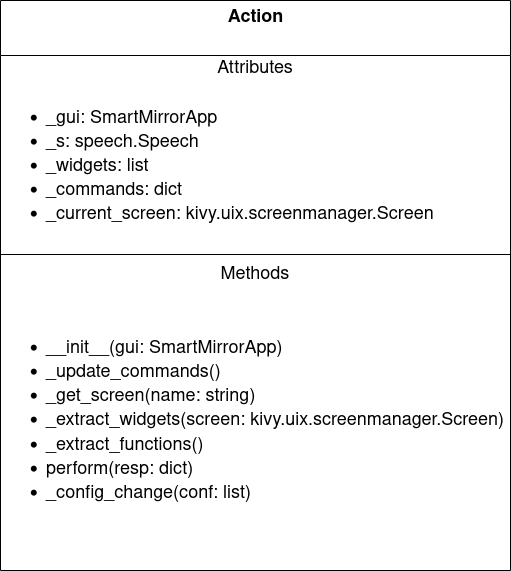
\includegraphics[scale=0.7]{images/uml_diagrams/Action.png}
    \caption{\engl{UML} της κλάσης \engl{Action}}
    \label{fig:action}
\end{figure}
\noindent\textbf{Περιγραφή Κλάσης}

Η κλάση αυτή αποτελεί την διεπαφή για την εκτέλεση των εντολών του χρήστη και είναι στην ουσία μια επέκταση του \engl{Controller}. Μέσω της συγκεκριμένης κλάσης, γίνεται η μετατροπή της πρόθεσης που παίρνει το σύστημα από το \engl{Wit.ai} σε εκτέλεση της κατάλληλης πράξης που υποδηλώνεται από την πρόθεση (αν αυτή υπάρχει και είναι προσβάσιμη).
\newpage
\noindent\textbf{Χαρακτηριστικά Κλάσης}
\begin{itemize}
    \item \engl{\texttt{\_gui}}: Αντικείμενο τύπου \engl{\texttt{SmartMirrorApp}} το οποίο χρησιμοποιείται για να γίνεται αλληλεπίδραση μεταξύ του \engl{Controller} και του γραφικού περιβάλλοντος.
    \item \engl{\texttt{\_s}}: Αντικείμενο τύπου \engl{\texttt{Speech}} το οποίο χρησιμοποιείται για την ομιλία του καθρέφτη προς τον χρήστη.
    \item \engl{\texttt{\_widgets}}: Μία λίστα που αποθηκεύει όλα τα \engl{Widgets} που βρίσκονται στην τωρινή οθόνη και το αντικείμενο \engl{\_gui}.
    \item \engl{\texttt{\_commands}}: Ένα \engl{dictionary} που αποθηκεύει τις δυνατές εντολές που εξάγει κάθε \engl{Widget} ως κλειδιά μαζί με τις αντίστοιχες συναρτήσεις που θα κληθούν για την κάθε εντολή ως τιμές.
    \item \engl{\texttt{\_current\_screen}}: Αντικείμενο τύπου \engl{kivy.uix.screenmanager.Screen} το οποίο έχει την τιμή της οθόνης στην οποία βρίσκεται κάθε στιγμή ο καθρέφτης.
\end{itemize}
\noindent\textbf{Μέθοδοι Κλάσης}
\begin{itemize}
    \item \engl{\texttt{\_\_init\_\_(gui: SmartMirrorApp)}}:
\end{itemize}

%%% Bibliography %%%
\printbibliography
\addcontentsline{toc}{chapter}{Βιβλιογραφία}

% Appendix
\chapter*{Παράρτημα}
\addcontentsline{toc}{chapter}{Παράρτημα}

\section{Μαθηματικοί Ορισμοί}\label{appendix:math_definitions}
\begin{definition}[Συνάρτηση \engl{argmax}]
\label{definition:argmax}
Δεδομένων ενός τυχαίου συνόλου \(X\), ενός συνόλου \(Y\) και μιας συνάρτησης \(f: X\rightarrow Y\), το μέγιστο όρισμα, \engl{argmax}, πάνω σε ένα υποσύνολο \(S \subseteq X\) ορίζεται ως
\[argmax_{S} \: f := \underset{x \in S}{argmax} f(x) := \{x \in S \: | \: f(s) \leq f(x)  \: \forall s \in S\} \]

Με άλλα λόγια, η συνάρτηση \engl{argmax} είναι το σύνολο των σημείων \(x\) για τα οποία η \(f(x)\) παίρνει την μέγιστη τιμή της.
\end{definition}

\begin{figure}[h]
\centering
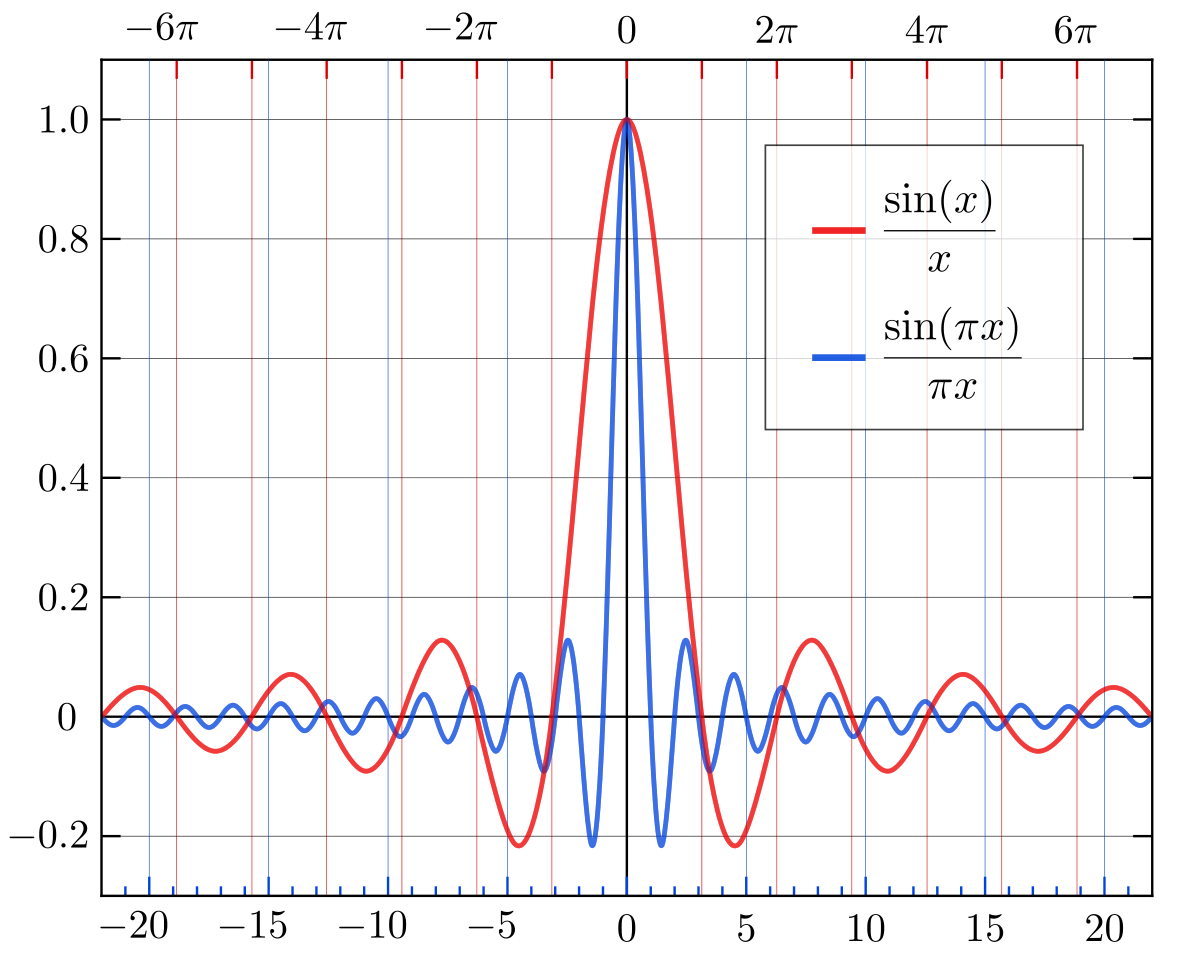
\includegraphics[scale=0.2]{images/3d_pose_estimation/function_argmax_example.png}
\caption[Παράδειγμα συνάρτησης \engl{argmax}]{Για παράδειγμα, οι συναρτήσεις \(sinc\) της γραφικής παράστασης έχουν και οι δύο \(argmax = 0\) επειδή έχουν μέγιστο το 1 στο \(x = 0\). }
\end{figure}

\begin{definition}[Συνάρτηση \engl{soft-argmax}]
\label{definition:soft-argmax}
Η συνάρτηση \engl{soft-argmax} \(f: \mathbb{R}^K  \rightarrow [0, 1)^K\) ορίζεται όταν \(\lVert K \rVert > 1\) ως

\(soft\_argmax = \sigma(\boldsymbol{x})_i := \frac{e^{x_i}}{\sum_{j=1}^{K}e^{x_j}}\) για \(i = 1,\cdots,K\) και \(\boldsymbol{x} = (x_1,\cdots,x_K) \in \mathbb{R}^K \)

\end{definition}

Ουσιαστικά, η συνάρτηση \engl{soft-argmax} εφαρμόζει την κανονική εκθετική συνάρτηση σε κάθε στοιχείο \(x_i\) του διανύσματος \(\boldsymbol{x}\) και κανονικοποιεί τις τιμές διαιρώντας με το άθροισμα όλων των εκθετικών. Η κανονικοποίηση αυτή εξασφαλίζει ότι το άθροισμα των στοιχείων του διανύσματος εξόδου \(\sigma(\boldsymbol{x})\) είναι 1.

\begin{definition}[Συνάρτηση \engl{ReLU}]
\label{definition:relu}
Η συνάρτηση \engl{ReLU} \(f: \mathbb{R} \rightarrow \mathbb{R}^+ \) ορίζεται ως

\( f(x) = max(0, x) \)

\end{definition}

H συνάρτηση \engl{ReLU} έχει ως έξοδο το όρισμα της όταν \(x > 0\), ενώ όταν \(x \leq 0\) η έξοδος είναι 0.

\begin{figure}[h]
\centering
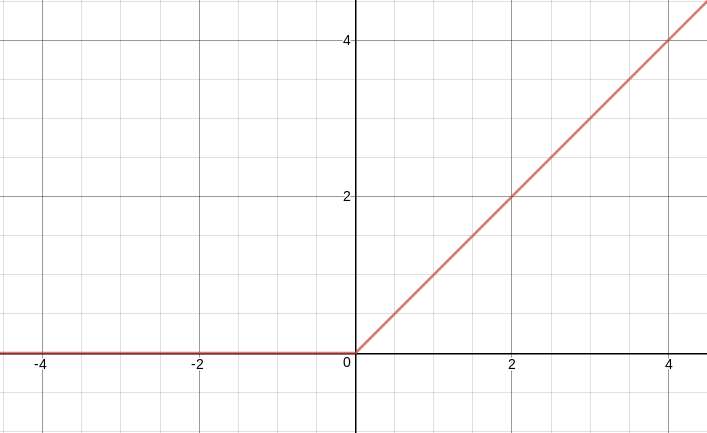
\includegraphics[scale=0.5]{images/3d_pose_estimation/relu_function.png}
\caption{H συνάρτηση \engl{ReLU}}
\end{figure}

\end{document}
